The empirical part is divided into blbnalanb

\section{Testing Configuration}
This section delves into the configuration and setup of our empirical testing. We begin by presenting our carefully selected datasets, which serve as the foundation for our evaluation. We highlight specific insights and characteristics of these datasets that make them compelling choices for our study. Afterward, we focus on the models we employ for testing and subsequent result comparison. We provide a comprehensive overview of the selected models, outlining their key features and motivations behind their inclusion in our evaluation. Subsequently, we provide a detailed description of the training pipeline and explain specific hyperparameters for which we will optimize these models.

\subsection{Datasets}\label{sec:datasets}
We will first explain our choice of datasets and introduce each dataset individually. Afterward, we will explore essential observations that are to be considered when assessing the actual empirical results.

\subsubsection{Choice of Datasets}
In selecting the datasets for our thesis, we adhered to two fundamental principles to ensure the robustness and diversity of our evaluation for \gnn and \wlnn models. The first principle focuses on using widely recognized benchmark datasets that have been extensively employed in previous studies. This principle enables us and readers to make meaningful comparisons with existing results. The second principle focuses on choosing datasets that are distinct from one another in terms of both their application domains and the way they encode information in graphs.

To fulfill the first principle, we opted for datasets from the TUDataset library. This library, curated by \cite{Mor+2020}, serves as a widely recognized standard for evaluating graph-related methods.

Regarding the second principle, we incorporated the insights from \cite{Liu2022}, who developed a comprehensive taxonomy of common graph benchmark datasets. Their work examined the degree to which information is encoded in graph structures compared to node features with respect to solving the task of the datasets. Based on their taxonomy, they categorized datasets into three distinct classes:
\begin{enumerate}
	\item Datasets in which the most crucial information for solving the task is contained in the node features.
	\item Datasets similar to the first category, but with the significant exception that the node degree strongly correlates with the node features. In these datasets, utilizing simple structural information, such as computing the node degree, is as beneficial for solving the task as using the original node features.
	\item Datasets where the most crucial information is encoded within the graph structure itself.
\end{enumerate}
These categories help us understand how information is encoded in various datasets, such that we aim to choose datasets from all three categories.

As a result of considering these two principles, we selected the following datasets for our thesis: \enzymes, \imdb, \mutag, \nci, \proteins, and \reddit for classification tasks, and \textsc{Alchemy} and \textsc{Zinc} for regression tasks. For an overview of the elemental properties of each dataset, see \cref{tab:overview_datasets}. We will now shortly introduce each dataset individually: \newline

\enzymes, provided by \cite{Borgwardt2005}, is a dataset consisting of proteins in their tertiary structure, categorized into six distinct enzyme classes. Each node represents a secondary structure, and has an edge to its three spatially closest nodes. Furthermore, each node feature encodes the type of secondary structure (\textit{helix}, \textit{sheet} or \textit{turn}), as well as physical and chemical information. \newline


\imdb, provided by \cite{Yanardag2015}, is a dataset comprising ego networks. Each node in the network represents an actor/actress, and a unidirectional edge exists between two nodes if and only if the corresponding actors played together in a movie. The task involves determining whether each ego network's genre is \textit{action} or \textit{romance}. \newline

\mutag, provided by \cite{Debnath1991}, is a dataset comprising Nitroaromatic compounds. Each compound is represented by a graph in which nodes represent atoms, with their types encoded as node features, and edges represent atomic bonds. The task involves determining whether a given compound has a mutagenic effect on Salmonella typhimurium bacteria. \newline

\nci, provided by \cite{Wale2008}, comprises graph representations of chemical compounds. In these graphs, nodes represent atoms, and edges represent atomic bonds. Moreover, the atom types are encoded in the node features. The overall task involves determining whether a given compound is active or inactive in inhibiting non-small cell lung cancer.\newline

\proteins, provided by \cite{Borgwardt2005}, contains proteins encoded similarly to \enzymes. The task here is to determine whether each graph represents an enzyme. \newline

\reddit, provided by \cite{Yanardag2015}, involves graphs that are derived from popular Reddit communities. The nodes in these graphs represent users who are active in the community, while the edges represent interactions between the users. The task is to identify whether a graph belongs to a community that is focused on questions and answers, or one that is focused on discussions. \newline

\textsc{Alchemy}, provided by \cite{Chen2019alchemy}, consists of organic molecules, with each node representing an atom and each edge representing an atomic bond. Additionally, each node feature encodes various properties for each atom, while each edge encodes the bond type and distance between atoms. The overall task is to compute 12 different continuous quantum mechanical properties for each graph. \newline

\textsc{Zinc}, provided by \cite{Bresson2019} and \cite{Irwin2012}, consists of molecular graphs where each node represents a heavy atom, and the corresponding node feature specifies its type. The edges in the graph encode the bonds between atoms, and their features further describe the type of bond. The task is to calculate a molecular property known as constrained solubility ($\log P - \text{SA} - \text{cycle}$).\newline

\begin{table}[!htb]
	\begin{center}
		\caption{Dataset statistics and properties for graph-level prediction tasks. This table has been adapted from \cite{Morris2022}.}
		\resizebox{0.975\textwidth}{!}{ 	\renewcommand{\arraystretch}{1.05}
			\begin{tabular}{@{}c <{\enspace}@{}lccccccc@{}}\toprule
				& \multirow{3}{*}{\vspace*{4pt}\textbf{Dataset}} & \multicolumn{7}{c}{\textbf{Properties}}\\
				\cmidrule{3-9}
				                         & & \shortstack{Number\\of graphs} & \shortstack{Number of\\classes/targets} & \shortstack{$\varnothing$ Number\\of nodes} & \shortstack{$\varnothing$ Number\\ of edges} & \shortstack{Node\\labels} & \shortstack{Edge\\labels} & \shortstack{Taxonomy \\Category} \\ \midrule
				\multirow{6}{*}{\rotatebox{90}{Classification}}
				& $\enzymes$       & 600               & 6                         & 32.6                          & 62.1                          & \cmark                   & \xmark  & 1    \\
				& $\imdb$   & 1\,000            & 2                         & 19.8                          & 96.5                          & \xmark                   & \xmark   & 3   \\
				& $\mutag$         & 188               & 2                         & 17.9                          & 19.8                          & \cmark                   & \xmark   & 2   \\
								
				& $\nci$          & 4\,110            & 2                         & 29.9                          & 32.3                          & \cmark                   & \xmark   & 3   \\
				& $\proteins$      & 1\,113            & 2                         & 39.1                          & 72.8                          & \cmark                   & \xmark  & 2    \\
				& $\reddit$ & 2\,000            & 2                         & 429.6                         & 497.8                         & \xmark                   & \xmark & 3     \\ 
				\midrule
				\multirow{2}{*}{\rotatebox{90}{Reg.}}
				& $\textsc{Alchemy}$       & 202\,579          & 12                        & 10.1                          & 10.4                         & \cmark                   & \cmark & -     \\
				& $\textsc{Zinc}$       & 249\,456          & 1                        & 23.1                         & 24.9                          & \cmark                   & \cmark & -     \\
				\bottomrule
			\end{tabular}}
		\label{tab:overview_datasets}
	\end{center}
\end{table}

\subsubsection{Analysis of the Datasets}
To ensure the reliability and fairness of our evaluation, one of our initial steps was to assess the balance of our selected datasets for classification. We employed the normalized Shannon index to evaluate the balance of a dataset, where a value close to $0$ indicates maximum imbalance, while a value close to $1$ signifies perfect balance. See \cref{sec:definition_shannon_index} in the Appendix for a formal definition of this metric.

\begin{table}[!htb]
	\caption{An overview of the normalized Shannon index calculated for each dataset.}
	\label{tab:shannon_index}
	\centering
    \resizebox{.975\textwidth}{!}{ 	\renewcommand{\arraystretch}{0.9}
		\begin{tabular}{@{}c <{\enspace}@{}lcccccc@{}}	\toprule
			& \multirow{3}{*}{\vspace*{4pt}}&\multicolumn{6}{c}{\textbf{Dataset}}\\\cmidrule{3-8}
			& & {\enzymes}          & {\textsc{Imdb-Multi}}  & {\mutag}           & {\nci}       & {\proteins}  & {\reddit}
			\\
			\toprule
			\multirow{1}{*}{} 	&
			Shannon index & 1 & 1 & 0.920 & 1 & 0.973 & 1 \\
			\bottomrule
		\end{tabular}}              
\end{table}

\Cref{tab:shannon_index} provides an overview of the normalized Shannon index computed for each selected classification dataset. Upon analyzing the data, we observed that all the datasets exhibit high balance, as all their values are close to $1$. This finding assures us that the datasets do not suffer significant class imbalances, which will remain important in the following section.

In addition to the balance of all datasets, another important aspect is understanding the upper bound of performance achievable by both \gnn and \wlnn models on these datasets. Unlike in other areas of machine learning where multilayer perceptron models can achieve near-perfect performance due to their universal approximation capabilities (\cite{Hornik1991}), \gnn and \wlnn models have inherent limitations on their expressiveness. This restriction stems from the fact that the expressiveness of the \wl algorithm limits the performance of both frameworks. In detail, if the \wl algorithm can not distinguish a pair of graphs in a dataset, then neither a \gnn nor a \wlnn model can.

While we have pointed out that the \wl algorithm is, in general, quite powerful in distinguishing pairs of graphs in \cref{sec:related_work}; we also explained that it is not complete. Therefore, assuming that \gnn or \wlnn models exist that can achieve almost perfect accuracy on all classification datasets is not reasonable. Thus, we calculated the theoretical maximum accuracy achievable by a perfect model for each dataset. In detail, we even investigated how many iterations of the \wl algorithm it takes to achieve this accuracy. For a comprehensive overview of the accuracies achievable on all datasets, please refer to \cref{tab:max_accuracies}. In this table, we have included the accuracy achievable when running the \wl algorithm for $0$ iterations, which essentially means taking the initial node features as the coloring for iteration $0$ and assessing the expressiveness of this initial coloring.

\begin{table}[!htb]
	\caption{An overview of the maximum theoretical classification accuracy achievable for each dataset based on the number of \wl iterations in percent. A hyphen ``-'' indicates that the maximum accuracy has converged with fewer iterations, implying that further iterations do not improve the accuracy.}
	\label{tab:max_accuracies}
    \resizebox{.975\textwidth}{!}{ 	\renewcommand{\arraystretch}{0.9}
		\begin{tabular}{@{}c <{\enspace}@{}lcccccc@{}}	\toprule
			& \multirow{3}{*}{\vspace*{4pt}\textbf{1-WL}}&\multicolumn{6}{c}{\textbf{Dataset}}\\\cmidrule{3-8}
			& & {\enzymes}         &  {\imdb}  & {\mutag}           & {\nci}       & {\proteins}  & {\reddit}
			\\
			\toprule
			\multirow{6}{*}{} 	&
			Iterations: $0$       &  81.4 & 60.6 & 93.1 & 91.3 & 91.9 & 83.9
			\\ 
			& Iterations: $1$    & 100.0 & 88.6 & 95.7 & 99.5 & 99.7 & 100.0
			\\
			& Iterations: $2$    & - & - & 99.5 & 99.8 & - & - 
			\\
			& Iterations: $3$   & - & - & 100.0 & 99.8 & - & - 
			\\
			& Iterations: $4$    & - & - & - & - & - & -
			\\
			\cmidrule{2-8}\morecmidrules\cmidrule{2-8}
			& Max Accuracy     & 100.0 & 88.6 & 100.0 & 99.8 & 99.7 & 100.0      
			\\
			\bottomrule
		\end{tabular}}              
\end{table}

Upon examining the results, we observe that all datasets exhibit perfect or near-perfect theoretical classification accuracies. This result makes interpreting results obtained from actual \wlnn or \gnn models later on more straightforward. Additionally, the accuracy achievable after each number of iterations provides a theoretical lower limit on the number of message-passing layers a \gnn must be composed of to be even capable of achieving this accuracy. 

We have conducted the same analyzes on additional datasets, as their results might be valuable to the reader. For these, see \cref{tab:max_accuracies_app} in the Appendix.


\subsection{Choice of Models}
In selecting our models, we aimed to use techniques that are relatively generic and not highly specialized for any of the datasets, such that insights we gain upon analyzing the model's performance can be generalized better. Consequently, we opted for a basic set of models to maintain simplicity and versatility.

\subsubsection{\wlnn Models}
Our primary consideration for the \wlnn models revolves around choosing an encoding function, as all other components are fixed. To keep things straightforward, we decided to employ encoding functions consisting of two main components. Firstly, an optional preprocessing step that operates on the colors computed by the \wl algorithm. Secondly, a basic pooling function for transforming the color histogram into a fixed-size vector.

In more detail, the optional preprocessing step involves a simple look-up table. If utilized, this step maps each color injectively to a vector in the range of $[-1, 1]^n$, where the value of $n$ is a hyperparameter. By encoding the color information into higher dimensions, this approach aims to enhance efficiency during subsequent processing steps. For the second step, the pooling component, we selected elementary functions such as elementwise \textsf{Max}, \textsf{Mean}, and Summation (\textsf{Sum}). In summary, each of the \wlnn models can be uniquely identified by their encoding functions; therefore, we will refer to each model by their encoding function as follows:
\begin{equation*}
	\textsf{Embedding}-\{\textsf{Max}, \textsf{Mean}, \textsf{Sum}\} \quad \text{or} \quad \{\textsf{Max}, \textsf{Mean}, \textsf{Sum}\},
\end{equation*}
where ``\textsf{Embedding}'' indicates the use of the optional preprocessing step.

\subsubsection{\gnn Models}\label{sec:gnn_model_choice}
As mentioned in the introduction to this section, our focus is on keeping the models basic. Hence, we opted for \gin by \cite{Xu2018}, \gcn by \cite{Kip+2017}, and \gat by \cite{Velivckovic2017} as the base architecture for the message-passing layers. Each of these architectures was chosen for specific reasons.

Firstly, we included \gin as an obvious candidate because it has been proven to be as expressive as the \wl algorithm. This characteristic makes it interesting when comparing it to \wlnn models.
Next, we also included \gcn based on its good empirical success in recent years. Furthermore, the insights provided by \cite{Nikolentzos2023} demonstrated that, in a certain sense, the node features computed by \gcn and \gin are similar, making \gcn a reasonable alternative to \gin in cases where the advantage of \gin's expressiveness is not needed.
Lastly, we added \gat as an alternative approach to the other two architectures. In detail, \cite{Nikolentzos2023} also showed that the node features computed by \gat are entirely different from those computed by \gin or \gcn.

Regarding the choice of \textsf{Readout} functions, we decided to utilize functions that are composed of two components. The first component is one of the elementwise pooling functions, such as \textsf{Max}, \textsf{Mean}, and \textsf{Sum}, to aggregate the information from a graph representation into a fixed-sized vector. Secondly, we incorporate a multilayer perceptron to process the aggregated information further, similarly to the \wlnn models.

In summary, each of the \gnn models can be uniquely identified by their \gnn architecture and the pooling function utilized; therefore, we will refer to each model by these two properties as follows:
\begin{equation*}
	{\{\gat, \gcn, \gin\}} - \{\textsf{Max}, \textsf{Mean}, \textsf{Sum}\}.
\end{equation*}

Note that the selection of the Readout function creates similarities between the \gnn and \wlnn models. These similarities play a crucial role in ensuring that any empirical differences observed between the two frameworks are not attributed to the utilization of more powerful techniques.

\subsection{Experimental Setup}

For the empirical testing, we took measures to ensure the reliability of our results in terms of hyperparameter configuration. Additionally, we aimed to ensure the reproducibility of the training pipeline for each model.

\subsubsection{Testing Procedure}

We started by conducting tests on the classification datasets, which serve as the basis for our evaluation. In our testing code, we employ a 10-fold cross-validation approach. Within this framework, we further partitioned the training data randomly, allocating \perc{10} of it for validation purposes. Consequently, each training iteration consisted of \perc{81} of the original dataset as the training set, \perc{9} as the validation set, and \perc{10} as the test set. We repeat this testing procedure five times to mitigate the influence of randomness on the model's performance. Ultimately, we recorded the mean accuracy on the test set along with its standard deviation as the primary performance metric of the model. Note that the use of standard cross-validation for generating the splits and the choice of mean accuracy as our primary metric is reasonable and justified as the datasets are highly balanced, as demonstrated in Section 2.

In the case of the regression datasets, we adopted a slightly different testing procedure. Due to their larger scale compared to the classification datasets, we opted for a more time-efficient approach. To achieve this, we utilized pre-existing training pipelines developed in \cite{Mor+2020} and \cite{Morris2022}. These pipelines use a fixed training, validation, and test split, accelerating the testing process. Similar to the classification datasets, we performed five runs for each model configuration and conducted a hyperparameter sweep for all model configurations. We record the mean absolute error and its standard deviation, as well as the mean logarithmic absolute error and its standard deviation across all runs. Furthermore, we test two splits for each regression dataset: one utilizing only 10\,000 samples for training, while the other split uses the entire training set. \todo{Say that due to these reasons our main focus in testing is on the classification datasets!}

\subsubsection{Hyperparameter Optimization}\label{sec:hyperparam}
To ensure the comparability of our results with other works and limit the number of hyperparameters requiring optimization, we followed standard practices when configuring our models. Detailed information on all hyperparameters, including the ones we optimized, can be found in \cref{tab:sweep_wlnn} for the \wlnn models used in classification tasks, \cref{tab:sweep_gnn} for the \gnn models employed in classification tasks, and \cref{tab:sweep_wlnn_reg} for the \wlnn models utilized in the regression task in the Appendix. We will shortly discuss the most critical parameters we optimized for:

Early in our investigations, we made a significant observation regarding the learning performance of \wlnn models. We noticed considerable performance discrepancies when comparing \wlnn models using the standard version of the \wl algorithm with the one from \gnn's. Consequently, we investigated the possibility of parametrizing the \wl algorithm to enhance control over the expressiveness of the colorings it computes. Specifically, we focused on two crucial parameters: 1) the number of iterations and 2) the usage of its convergence behavior as an early termination criterion.

The advantage of this more granular parametrization is that it enables us to apply the same number of \wl iterations to each graph processed by a \wlnn model by deactivating the convergence behavior and fixing the number of iterations. By deactivating this behavior and keeping the number of iterations minimal, we observed that the number of colors used by the \wl algorithm remained contained. As a result, the \mlp component of each \wlnn model seems to generalize better, significantly improving performance. Therefore, one of the most crucial hyperparameters we optimized for all \wlnn models was the number of \wl iterations. Additionally, if employed, the size of the dimension of the look-up table was another significant parameter to optimize.

In contrast, the hyperparameter selection for the \gnn models was relatively less intricate. The key parameters of interest here are the number of message-passing layers and the size of the hidden dimensions used in each layer. The reason for this is that the number of layers directly corresponds to the expressiveness of the \gnn, as demonstrated in the proof, while the size of the hidden dimensions enables easier learning by allowing the model to store more information during graph processing.

\subsubsection{Implementation Details and Result Accessibility}
The implementation of our models and training procedures was carried out using \textsc{Python 3.10} along with the open-source library \textsc{PyTorch}\footnote{A free and open-source machine learning framework that was originally developed by Meta AI and is now part of the Linux Foundation umbrella. \href{https://pytorch.org}{https://pytorch.org}} and its extension \textsc{PyTorch Geometric}\footnote{An open-source library that extends \textsc{PyTorch} and allows for easy development and training of graph neural networks. \href{https://pytorch-geometric.readthedocs.io/en/latest}{https://pytorch-geometric.readthedocs.io}}. Moreover, we leveraged \textsc{Weights\&Biases} as our tool for coordinating and recording the results of the hyperparameter optimization. The code for our experiments is publicly available on \textsc{GitHub} at \url{https://github.com/ericbill21/BachelorThesis}, and the corresponding results can be accessed via \textsc{Weights\&Biases} at \url{https://wandb.ai/eric-bill/BachelorThesisExperiments}. We conducted our tests on the RWTH High Performance Computing cluster by the RWTH Aachen University as well as on private hardware.

\section{Empirical Testing}
In this section, we present the empirical findings of our study. A total of 5\,581 runs were conducted, with each run testing a specific model configuration on a designated dataset. These runs required a substantial amount of computation time, totaling 1\,644 hours (over 70 days). To examine the classification accuracy achieved by the best-performing configuration of each model on each classification dataset, please refer to \cref{tab:results_classification}. For regression datasets, \cref{tab:results_regression} provides an overview of the mean absolute error (MAE) for the best-performing configurations.

Due to the significantly larger size of the regression datasets compared to the classification datasets, running regression experiments required considerable time for each configuration. As a result, we had to limit the number of different configurations tested. For this reason, we employed existing training pipelines, as mentioned in the previous section, which allowed us to include the results of the \gineeps model proposed by \cite{Mor+2020} and \cite{Morris2022} in \cref{tab:results_regression}.
The \gineeps model utilizes the \gin architecture for message-passing layers, \textsf{Mean} as its pooling function, and a two-layer \mlp for the final processing of its input graph. This design closely resembles our \textsf{GIN:Mean} model, with the crucial distinction being that \gineeps incorporates edge features in its computations.

The decision to exclude edge features from all our models, including all \wlnn models, was driven by two key factors. Firstly, our focus primarily revolved around the classification datasets, all of which do not encode any information in their edge features (refer to \cref{tab:overview_datasets}). Secondly, the regression datasets we utilized in our evaluation include continuous edge features, making the application of the \wl algorithm more complex. Although some work exists on modifying the \wl algorithm to incorporate continuous features, we opted for a more straightforward and more scalable approach by not considering edge features in the computations of all our models. Nonetheless, this limitation does not compromise the integrity of our results, as our main objective is to compare similar \gnn and \wlnn models. The inclusion of \gineeps showcases the potential and highlights the significance of edge feature information for solving the dataset tasks of \textsc{Alchemy} and \textsc{Zinc}.

A notable finding when analyzing the presented results is that the performance of \wlnn models is comparable to that of \gnn models. In fact, the best \wlnn models even outperform the \gnn models in all classification datasets, with the exception of \imdb and \reddit. These two datasets stand out among the classification datasets as they lack node features. We will investigate this insight later on in more detail. 
Moreover, our results align with the empirical findings of other \gnn models in various studies. The accuracy reported here falls within a similar range as observed in works by \cite{Xu2018,Morris2022,Mor+2020,Zhang2018}. 

In the subsequent subsection, we will further analyze these results. Specifically, we will investigate the tradeoff between generality and expressiveness in \wlnn models, the learned aggregation functions of each model, the ability of \gnn models to approximate \wlnn models, the differences in their learning behaviors, and the impact of \gnn models performance by preprocessing the data.

\begin{table}[!htb]
	\caption{Overview of the mean classification accuracies achieved by the best configuration of each model for each dataset in percent and standard deviation.}
	\label{tab:results_classification}
    \resizebox{.975\textwidth}{!}{ 	\renewcommand{\arraystretch}{1.05}
		\begin{tabular}{@{}c <{\enspace}@{}lcccccc@{}}	\toprule
			& \multirow{3}{*}{\vspace*{4pt}\textbf{Method}}&\multicolumn{6}{c}{\textbf{Dataset}}\\\cmidrule{3-8}
			& & {\enzymes}         &  {\imdb}      & {\mutag}           & {\nci}       & {\proteins}           & 
			{\reddit}
			\\
			\toprule
			\multirow{6}{*}{\rotatebox{90}{$\wlnn$}} 	&
			\textsf{Max} & 16.7 \scriptsize $\pm 4.2$ & 52.0 \scriptsize $\pm 5.3$	&73.8 \scriptsize $\pm 12.4$ &	58.6 \scriptsize $\pm 3.3$ & 62.9 \scriptsize $\pm 4.9$  & 	69.2 \scriptsize $\pm 4.0$
			\\ 
			& \textsf{Mean} & 18.2 \scriptsize $\pm 4.8$  &	59.4 \scriptsize $\pm 5.8$ &	77.1 \scriptsize $\pm 11.5$	 & 64.0 \scriptsize $\pm 3.3$ &	60.9 \scriptsize $\pm 4.5$ & 66.1 \scriptsize $\pm 3.2$   
			\\ 	
			& \textsf{Sum} & 18.0 \scriptsize $\pm 6.2$	 & 57.5 \scriptsize $\pm 5.1$ & 66.8 \scriptsize $\pm 13.9$ & 56.9 \scriptsize $\pm 3.8$ & 65.6 \scriptsize $\pm 4.8$ & 73.0 \scriptsize $\pm 5.1$   
			\\  
			\cmidrule{2-8}  		
			& \textsf{Embedding-Max} & 40.5  \scriptsize	$\pm 7.4$         & 69.4  \scriptsize $\pm 4.9$             & 81.1 \scriptsize $\pm 11.2$	 & 82.7  \scriptsize $\pm 2.0$          & \textbf{75.2} \scriptsize $\pm 3.9$ & 71.1 \scriptsize $\pm 3.9$    
			\\ 
			& \textsf{Embedding-Mean}     & 42.6 \scriptsize	$\pm 9.0$ & \textbf{72.4}     \scriptsize $\pm 4.1 $         & 84.1 \scriptsize $\pm 9.1$	       & 83.1   \scriptsize $\pm 1.9$         & 72.3  \scriptsize $\pm 4.2$ & 75.4 \scriptsize $\pm 2.8$
			\\ 
			& \textsf{Embedding-Sum} & \textbf{48.3} \scriptsize	$\pm 8.1$          & 72.0  \scriptsize $\pm 3.8$             & \textbf{85.1} \scriptsize $\pm 8.6$	     & \textbf{83.6}   \scriptsize $\pm 2.2$         & 75.2  \scriptsize $\pm 4.5$ & \textbf{78.4} \scriptsize $\pm 2.7$    
			\\ 
			\cmidrule{2-8}
			\multirow{9}{*}{\rotatebox{90}{Graph Neural Networks}} 
			& \textsf{GAT:Max}                    & 31.2 \scriptsize $\pm 6.0$        & 70.7 \scriptsize $\pm 4.8$          & 71.1 \scriptsize $\pm 12.2$ & 58.0 \scriptsize $\pm 4.2$          & 72.5 \scriptsize $\pm 5.1$         & 77.7 \scriptsize $\pm 5.0$ 
			\\ 
			& \textsf{GAT:Mean}    & 28.9 \scriptsize $\pm 5.9$          & 70.9 \scriptsize $\pm 3.7$           & 74.8 \scriptsize $\pm 9.1$            & 66.1 \scriptsize $\pm 2.8$         & 64.9 \scriptsize $\pm 6.4$  & 70.0 \scriptsize $\pm 6.9$
			\\ 
			& \textsf{GAT:Sum}                  & \textbf{34.4} \scriptsize $\pm 7.0$          & 72.2 \scriptsize $\pm 4.5$	            & 82.1 \scriptsize $\pm 11.2$            & 69.8 \scriptsize $\pm 2.6$	          & 73.4 \scriptsize $\pm 3.9$ & 78.1 \scriptsize $\pm 4.2$        
			\\
			\cmidrule{2-8}
			& \textsf{GCN:Max} & 33.1 \scriptsize $\pm 7.5$ &	73.5 \scriptsize $\pm 4.1$	& 74.5 \scriptsize $\pm 11.3$ & 61.1 \scriptsize $\pm 3.6$ &	69.8 \scriptsize $\pm 5.9$ & 74.3 \scriptsize $\pm 4.5$
			\\ 
			& \textsf{GCN:Mean} & 29.9 \scriptsize $\pm 5.7$ &	\textbf{74.7} \scriptsize $\pm 3.8$ & 75.0 \scriptsize $\pm 10.4$ &	68.9 \scriptsize $\pm 2.4$ &	70.9 \scriptsize $\pm 5.2$ & 82.3 \scriptsize $\pm 3.3$
			\\ 
			& \textsf{GCN:Sum} & 31.7 \scriptsize $\pm 7.2$ &	73.0 \scriptsize $\pm 4.4$	& 81.5 \scriptsize $\pm 10.3$ & 70.4 \scriptsize $\pm 2.1$ & 3.5 \scriptsize $\pm 3.9$ & \textbf{86.9} \scriptsize $\pm 3.2$                       
			\\
			\cmidrule{2-8}	
						
			& \textsf{GIN:Max} & 29.2 \scriptsize $\pm 6.2$	& 70.8 \scriptsize $\pm 4.7$ & 77.3 \scriptsize $\pm 10.7$ & \textbf{79.9} \scriptsize $\pm 2.2$ & \textbf{74.3} \scriptsize $\pm 5.1$ & 76.1 \scriptsize $\pm 3.6$  
			\\ 
			& \textsf{GIN:Mean}  & 31.7 \scriptsize $\pm 6.7$	& 71.1 \scriptsize $\pm 5.4$ & 82.4 \scriptsize $\pm 9.8$ & 	70.8 \scriptsize $\pm 2.2$ & 72.0 \scriptsize $\pm 4.0$ & 73.5 \scriptsize $\pm 3.8$
			\\ 
			& \textsf{GIN:Sum} & 28.9 \scriptsize $\pm 8.7$ & 	69.5 \scriptsize $\pm 4.8$	& \textbf{84.6} \scriptsize $\pm 8.7$ & 70.8 \scriptsize $\pm 2.3$ & 74.0 \scriptsize $\pm 4.3$ & 74.0 \scriptsize $\pm 4.3$
			\\
			\bottomrule
		\end{tabular}}            
\end{table}

\begin{table}[!htb]
	\caption{Overview of the mean absolute error and the standard deviation (logMAE) on large-scale (multi-target) molecular regression tasks. The results marked by $^1$ are adopted from \cite{Mor+2020} and by $^2$ from \cite{Morris2022}.}
	\resizebox{0.975\textwidth}{!}{ 	\renewcommand{\arraystretch}{1.05}
	\newcommand{\seq}[2]{$(#1, #2)$\text{-}\textsf{SpeqNet}\xspace}
		\begin{tabular}{@{}c <{\enspace}@{}lcccc@{}}	\toprule
			& \multirow{3}{*}{\vspace*{4pt}\textbf{Method}}&\multicolumn{4}{c}{\textbf{Dataset}}
			\\
			\cmidrule{3-6}
			& & {\textsc{Alchemy}} & {\textsc{Alchemy (10k)}} & {\textsc{Zinc}} & {\textsc{Zinc (10k)}} 
			\\	
			\toprule
			\multirow{4}{*}{\rotatebox{90}{\gnn}} 
			& \textsf{$\gineeps^{1,2}$} & 0.103 {\scriptsize $\pm  0.001$} -2.956 {\scriptsize $\pm  0.029$}$^1$ & 0.180 {\scriptsize $\pm  0.006$} -1.958  {\scriptsize $\pm  0.047$}$^2$ & - & 0.084 {\scriptsize $\pm  0.004$}$^1$
			\\
			\cmidrule{2-6}
			& \textsf{GIN:Max} & 0.604 {\scriptsize $\pm 0.004$} -0.578 {\scriptsize $\pm 0.009$} &	0.353 {\scriptsize $\pm 0.003$} -1.228 {\scriptsize $\pm 0.006$} &	0.124 {\scriptsize $\pm 0.004$} &	0.427 {\scriptsize $\pm 0.009$}
			\\
			& \textsf{GIN:Mean} & 0.643 {\scriptsize $\pm 0.014$} -0.505 {\scriptsize $\pm 0.021$} & 0.314 {\scriptsize $\pm 0.004$} -1.469 {\scriptsize $\pm 0.044$} & 0.110 {\scriptsize $\pm 0.005$} & 0.341 {\scriptsize $\pm 0.037$}
			\\
			& \textsf{GIN:Sum} & \textbf{0.523} {\scriptsize $\pm 0.016$} -0.705 {\scriptsize $\pm 0.035$} & \textbf{0.282} {\scriptsize $\pm 0.002$} -1.890 {\scriptsize $\pm 0.031$} & \textbf{0.104} {\scriptsize $\pm 0.005$} & \textbf{0.298} {\scriptsize $\pm 0.034$}
			\\
			\cmidrule{2-6}
			\multirow{3}{*}{\rotatebox{90}{\scriptsize \wlnn}} 
			& \textsf{Embedding-Max} & 0.648 {\scriptsize $\pm 0.003$} -0.511 {\scriptsize $\pm 0.009$} &	0.409 {\scriptsize $\pm 0.003$} -1.023 {\scriptsize $\pm 0.009$} &	0.382 {\scriptsize $\pm 0.005$} &	0.659 {\scriptsize $\pm 0.007$}
			\\
			& \textsf{Embedding-Mean} & 0.617 {\scriptsize $\pm 0.003$} -0.564 {\scriptsize $\pm 0.005$} &	0.355 {\scriptsize $\pm 0.004$} -1.269 {\scriptsize $\pm 0.020$} &	\textbf{0.348} {\scriptsize $\pm 0.010$} &	0.484 {\scriptsize $\pm 0.009$}
			\\
			& \textsf{Embedding-Sum} & \textbf{0.600} {\scriptsize $\pm 0.004$} -0.625 {\scriptsize $\pm 0.032$} & \textbf{0.305} {\scriptsize $\pm 0.001$} -1.740 {\scriptsize $\pm 0.042$} &	0.384 {\scriptsize $\pm 0.004$} &	\textbf{0.465} {\scriptsize $\pm 0.009$}
			\\
			\bottomrule
	\end{tabular}}
	\label{tab:results_regression}
\end{table}


\subsection{Fixed \wl Iterations: Tradeoff between Expressiveness and Generality}
As discussed in Section \ref{sec:hyperparam}, we explored constraining the expressiveness of the \wl algorithm by fixing the number of iterations it is applied to each graph in a \wlnn model. The intention behind this was to ensure that the resulting colorings of graphs computed using a fixed \wl algorithm would fall within a similar color range, thereby limiting the total number of colors and avoiding outlier cases.

From a theoretical perspective, fixing the number of \wl iterations in a \wlnn model only limits its expressiveness. For the remainder of this section, we will denote the number of \wl iterations by $\nwl \in \Nb$.
For instance, let $\nwl \in \Nb$ now be fixed. If the standard \wl algorithm converges on an input graph $G$ after $k' < k$ iterations, the coloring computed after $\nwl$ iterations is as expressive as the one obtained from the standard \wl algorithm since the coloring convergence after $k'$ iterations. On the contrary, if the standard \wl algorithm converges after $k' > k$ iterations on an input graph $G$, the coloring obtained after $\nwl$ iterations is less expressive and contains less information than the coloring derived from the standard \wl algorithm.

Comparing the performance of \wlnn models utilizing the standard \wl algorithm to those using the parametrized version reveals a significant difference across all classification datasets, as seen in \cref{tab:wl_parametrization}. This data confirms our belief that the standard \wl algorithm can be overly expressive for specific tasks, as evidenced by the considerable performance gap between the two types of the algorithm. Additionally, we included the mean number of iterations of the \wl algorithm applied on each dataset graph in the brackets in Table 4. This number remains a fixed constant for the models utilizing the parametrized version.

\begin{table}[!htb]
    \resizebox{.975\textwidth}{!}{ 	\renewcommand{\arraystretch}{1.05}
		\begin{tabular}{@{}c <{\enspace}@{}lcccccc@{}}	\toprule
			\multicolumn{2}{c}{\multirow{2}{*}{\textbf{Algorithm Type}}} &\multicolumn{6}{c}{\textbf{Dataset}}\\\cmidrule{3-8}
			& & {\enzymes}         &  {\imdb}      & {\mutag}           & {\nci}       & {\proteins}           & 
			{\reddit}
			\\
			\toprule
			\multirow{2}{*}{\textbf{Standard}}
			& Test Accuracy: & 34.2 {\scriptsize $\pm 6.7$} & 67.0 {\scriptsize $\pm 4.3$} & 76.3 {\scriptsize $\pm 9.4$} & 78.9 {\scriptsize $\pm 2.1$} & 71.4 {\scriptsize $\pm 4.9$} & 70.9 {\scriptsize $\pm 3.8$}
			\\
			& $\varnothing$ \wl Iterations: & 3.0 {\scriptsize $\pm 1.7$} &  1.1 {\scriptsize $\pm 0.7$} & 4.2 {\scriptsize $\pm 1.6$} & 3.9 {\scriptsize $\pm 1.7$} & 3.0 {\scriptsize $\pm 1.7$} & 4.1 {\scriptsize $\pm 0.9$}\\
			\cmidrule{2-8}
			\multirow{2}{*}{\textbf{Parametrized}}
			& Test Accuracy: & 48.3 {\scriptsize $\pm 8.1$} & 72.4 {\scriptsize $\pm 4.1$} & 85.1 {\scriptsize $\pm 8.6$} & 83.6 {\scriptsize $\pm 2.2$} & 75.2 {\scriptsize $\pm 3.9$} & 78.4 {\scriptsize $\pm 2.7$}
			\\
			& \# \wl Iterations: & 1 & 1 & 1 & 3 & 1 & 1 \\
			\bottomrule
		\end{tabular}}
		\caption{Comparison between the best performing \wlnn models using the standard \wl algorithm and the one employing the parametrized version of it in percent and standard deviation. Additionally, we put the average number of iterations of the \wl algorithm in brackets for each model.}
        \label{tab:wl_parametrization}     
\end{table}

Building on these insights, investigating the optimal number of \wl iterations that lead to the best-performing models is another interesting observation. To illustrate its effect, we created \cref{fig:k_wl_dependence}, which showcases the performance achieved by all models and configurations grouped by the number of \wl iterations for each dataset in a violin graph. Note that both classification and regression datasets are included in this figure. Depending on the dataset type, the y-axis represents either classification accuracy or test error, where higher accuracies imply better performance for classification tasks, and higher test errors imply poorer performance for regression tasks (and vice versa).

In general, the results indicate that the performance of \wlnn models tends to improve as the number of \wl iterations decreases, except for \nci, \textsc{Alchemy} and \textsc{Zinc} datasets. 

Notably, for \nci, the optimal number of iterations coincides with the number of \wl iterations needed for the maximum achievable accuracy (refer to \cref{tab:max_accuracies}). This correlation holds for all other classification datasets, except for \mutag. However, the behavior observed in \mutag can potentially be attributed to the fact that according to the introduced taxonomy (\cite{Liu2022}) in Section \ref{sec:datasets}, \mutag can be effectively solved by simply replacing its node features with an encoding of the node degree. Since, from a theoretical perspective, the coloring computed after the first iteration of the \wl algorithm is usually an encoding of the node degree, this might explain the observed pattern.

Interpreting the results of the \textsc{Zinc} dataset is more complex and somewhat peculiar. While the smaller subset of the dataset, \textsc{Zinc10K}, clearly indicates that fewer \wl iterations yield better results, the overall \textsc{Zinc} dataset suggests the opposite. This discrepancy could be attributed to the limited number of runs conducted on the entire dataset, which were restricted due to scalability and time constraints. Therefore, these results should be interpreted with caution.

In conclusion, reducing the number of \wl iterations leads to improved generability and overall better performance of the models, with the clear exception of \nci. However, as our results indicate, most \wlnn models achieve optimal performance when employing only a single iteration of the \wl algorithm, which is essentially equivalent to encoding the node degree. This observation demonstrates that \wlnn models do not require the full expressiveness of the \wl algorithm to achieve comparable performance to \gnn models, which raises the question of whether \gnn models, despite their theoretical ability to be highly expressive, also tend to rely primarily on node degree information for computation. We will explore this question further in Section TODO.

\begin{figure}[!htb]
	\centering
	\begin{subfigure}[b]{0.19\textwidth}
		\centering
		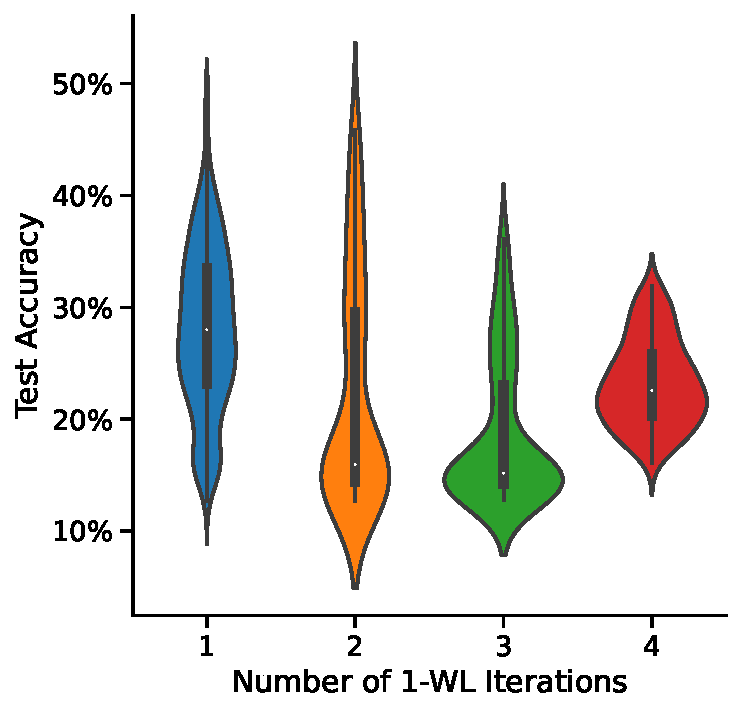
\includegraphics[width=\textwidth]{Figures/k_wl_violin_ENZYMES.pdf}
        \caption{\scriptsize\enzymes}
	\end{subfigure}
	\hfill
	\begin{subfigure}[b]{0.19\textwidth}
		\centering
		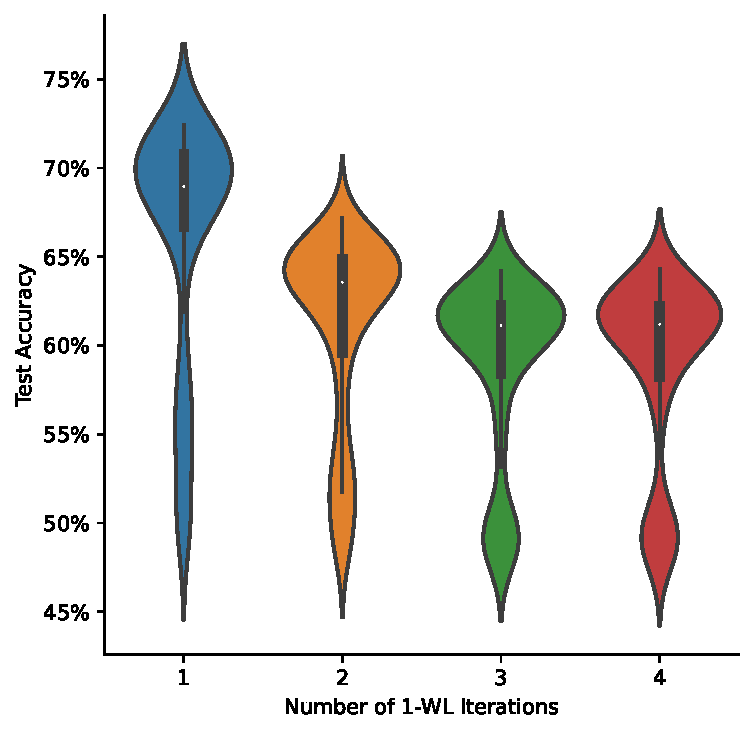
\includegraphics[width=\textwidth]{Figures/k_wl_violin_IMDB-BINARY.pdf}
        \caption{\scriptsize\imdb}
	\end{subfigure}
	\hfill
	\begin{subfigure}[b]{0.19\textwidth}
		\centering
		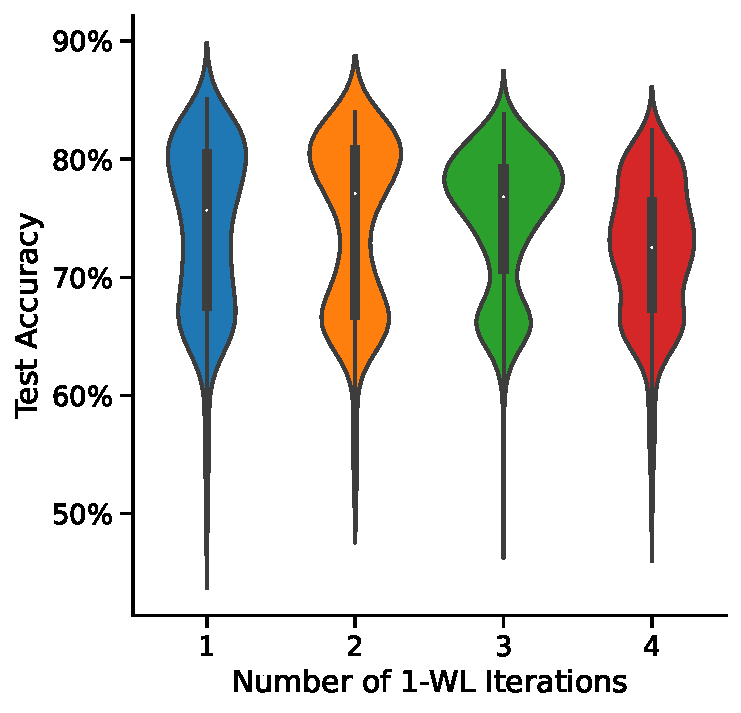
\includegraphics[width=\textwidth]{Figures/k_wl_violin_MUTAG.pdf}
        \caption{\scriptsize\mutag}
	\end{subfigure}
	\hfill
	\begin{subfigure}[b]{0.19\textwidth}
		\centering
		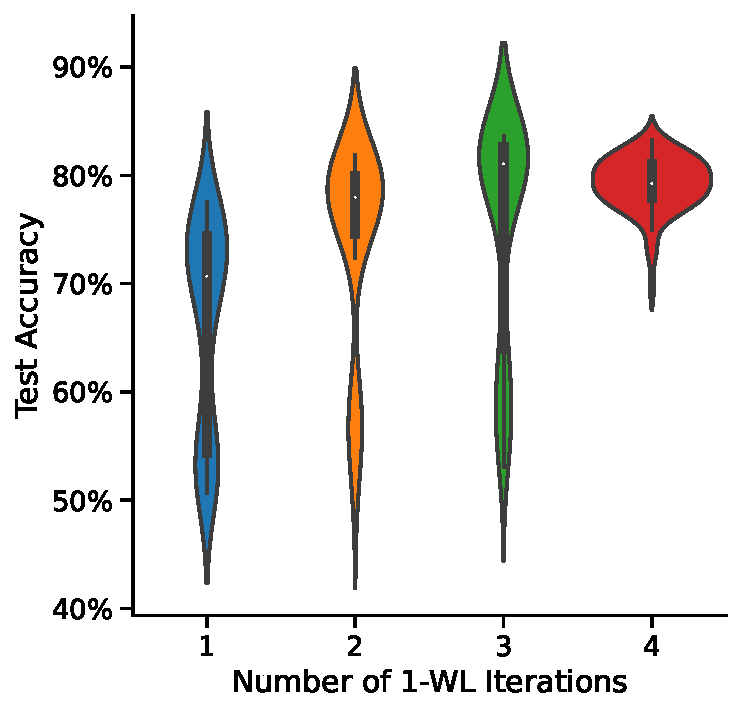
\includegraphics[width=\textwidth]{Figures/k_wl_violin_NCI1.pdf}
        \caption{\scriptsize\nci}
	\end{subfigure}
	\hfill
	\begin{subfigure}[b]{0.19\textwidth}
		\centering
		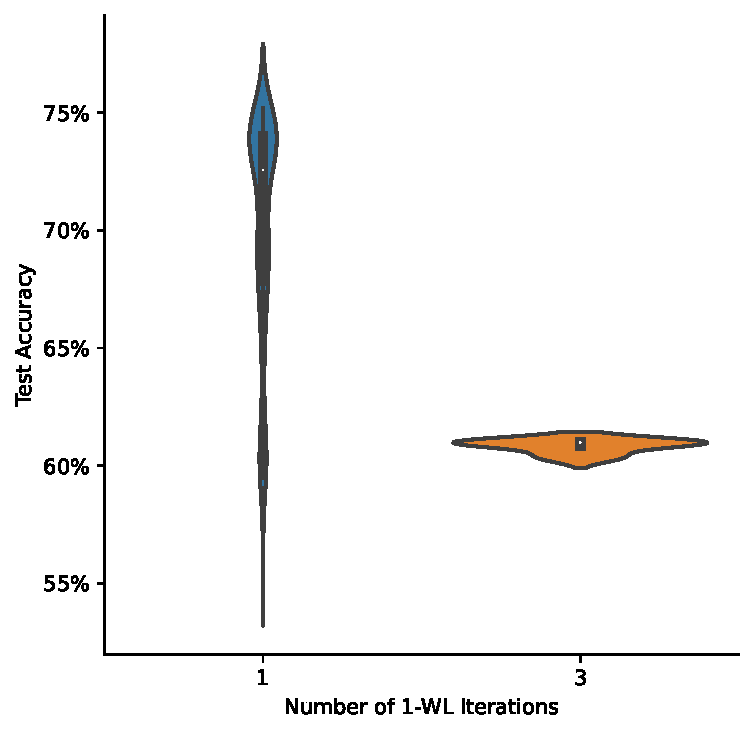
\includegraphics[width=\textwidth]{Figures/k_wl_violin_PROTEINS.pdf}
        \caption{\scriptsize\proteins}
	\end{subfigure}
	\par\bigskip
	\begin{subfigure}[b]{0.19\textwidth}
		\centering
		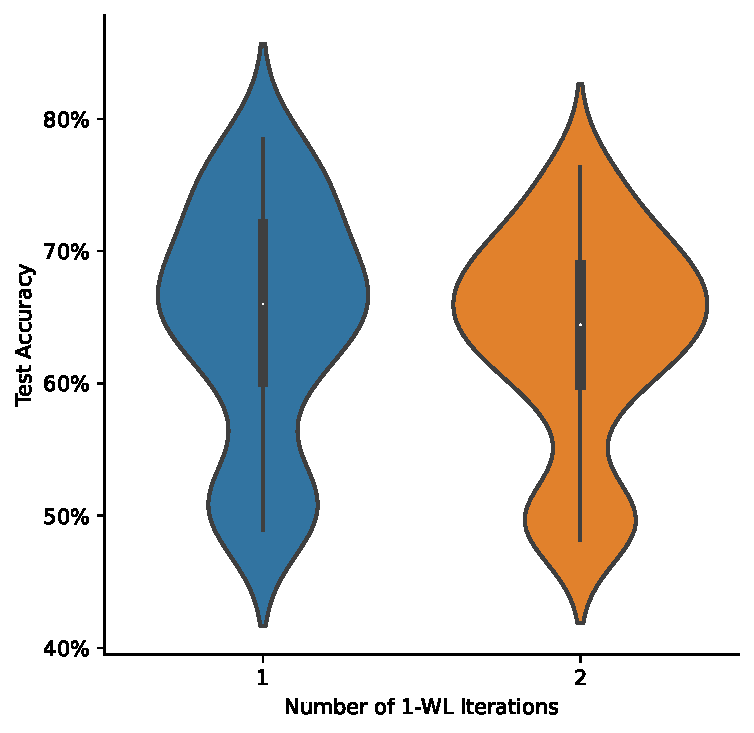
\includegraphics[width=\textwidth]{Figures/k_wl_violin_REDDIT-BINARY.pdf}
        \caption{\scriptsize \reddit}
	\end{subfigure}
	\hfill
	\begin{subfigure}[b]{0.19\textwidth}
		\centering
		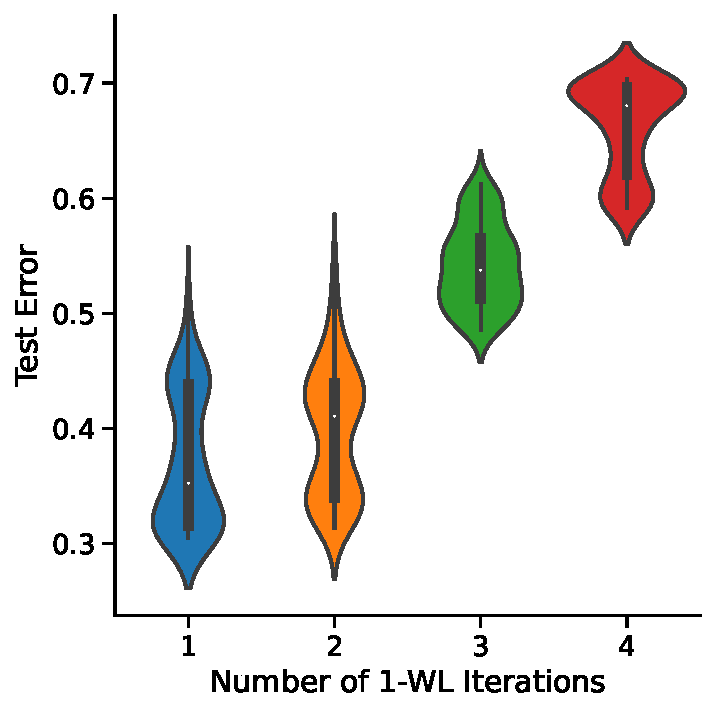
\includegraphics[width=\textwidth]{Figures/k_wl_violin_Alchemy10K.pdf}
        \caption{\scriptsize\textsc{Alchemy (10k)}}
	\end{subfigure}
	\hfill
	\begin{subfigure}[b]{0.19\textwidth}
		\centering
		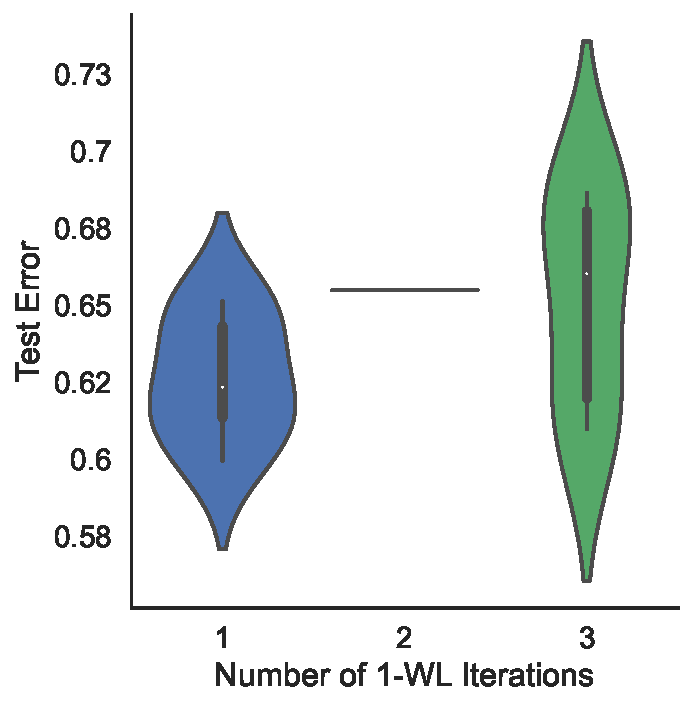
\includegraphics[width=\textwidth]{Figures/k_wl_violin_Alchemy.pdf}
        \caption{\scriptsize\textsc{Alchemy}}
	\end{subfigure}
	\hfill
	\begin{subfigure}[b]{0.19\textwidth}
		\centering
		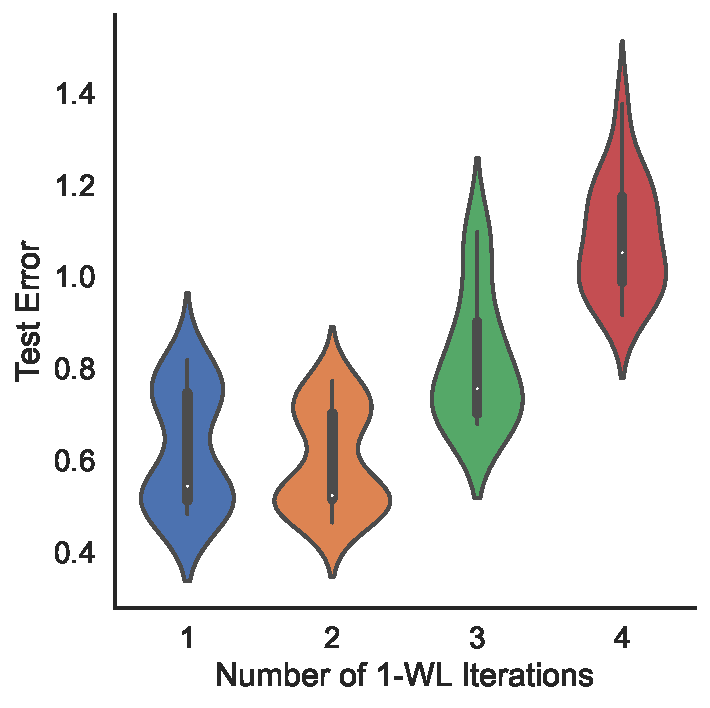
\includegraphics[width=\textwidth]{Figures/k_wl_violin_Zinc 10k.pdf}
        \caption{\scriptsize\textsc{Zinc (10k)}}
	\end{subfigure}
	\hfill
	\begin{subfigure}[b]{0.19\textwidth}
		\centering
		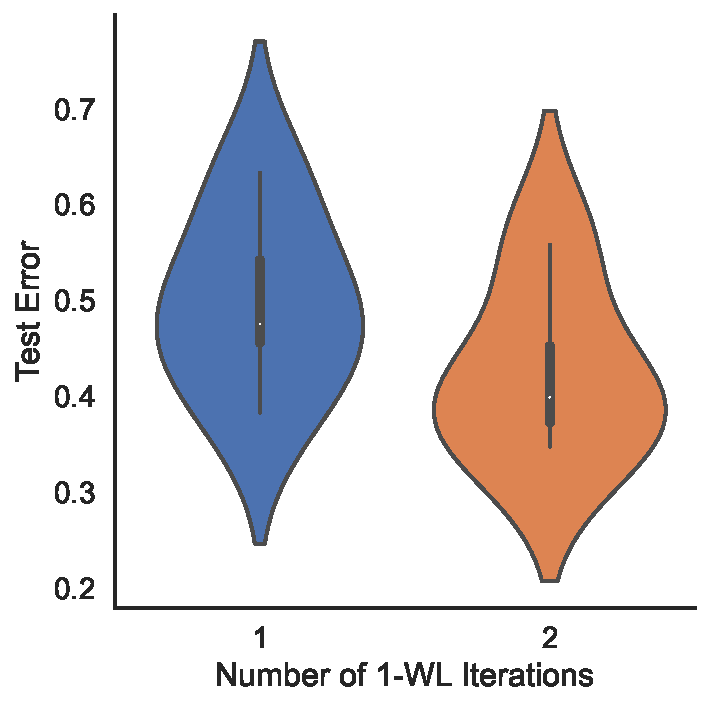
\includegraphics[width=\textwidth]{Figures/k_wl_violin_Zinc.pdf}
        \caption{\scriptsize\textsc{Zinc}}
	\end{subfigure}
	\caption{Impact on performance by the number of itertations of the \wl alogirhtm.}
	\label{fig:k_wl_dependence}
\end{figure}


\subsection{Difference in Learning behavior}
The learning behavior of \wlnn models presents a unique challenge due to the expressiveness of the \wl algorithm, which directly impacts their performance. Compared to \gnn models, \wlnn models exhibit a significant discrepancy between their training and test performance. While it is common to observe higher training performance than testing performance in various machine learning applications, this discrepancy is particularly pronounced in our evaluation of the \wlnn models.

\cref{fig:performance_diff} visually represents the difference in performance between the training and testing performance for both \wlnn and \gnn models across all classification datasets. Different quantiles from the best-performing models were considered, ranging from the top \perc{1} to the top \perc{100}. Each bar in the graph represents the mean difference between training accuracy and test accuracy for the respective quantile of runs. \wlnn models are depicted in blue, while \gnn models are represented in orange. In comparison, shorter or negative bars indicate better generalization where the performance on the training set aligns more closely with the testing set. The black line in each bar represents the standard error.

\begin{figure}[!htb]
	\begin{subfigure}[b]{0.3\textwidth}
		\centering
		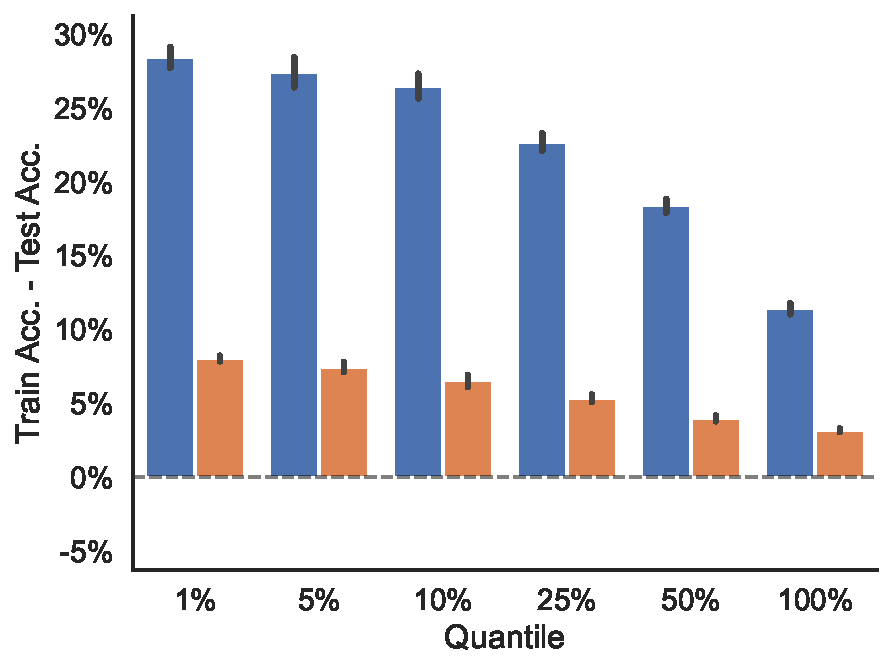
\includegraphics[width=\textwidth]{Figures/train_test_diff_ENZYMES.pdf}
		\vspace*{-4ex} 
		\caption{\enzymes}
	\end{subfigure}
	\hfill
	\begin{subfigure}[b]{0.3\textwidth}
		\centering
		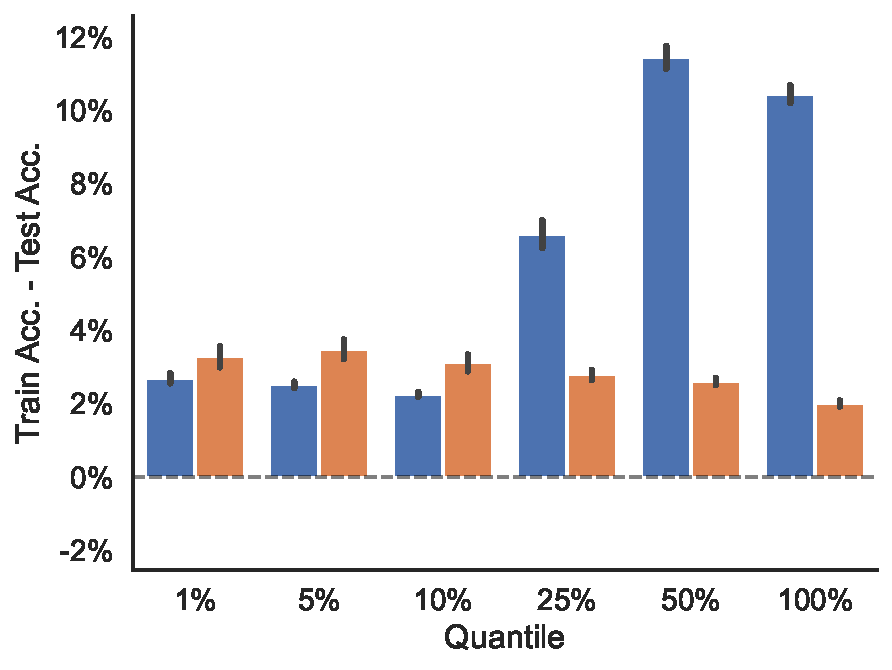
\includegraphics[width=\textwidth]{Figures/train_test_diff_IMDB-BINARY.pdf}
		\vspace*{-4ex} 
		\caption{\imdb}
	\end{subfigure}
	\hfill
	\begin{subfigure}[b]{0.3\textwidth}
		\centering
		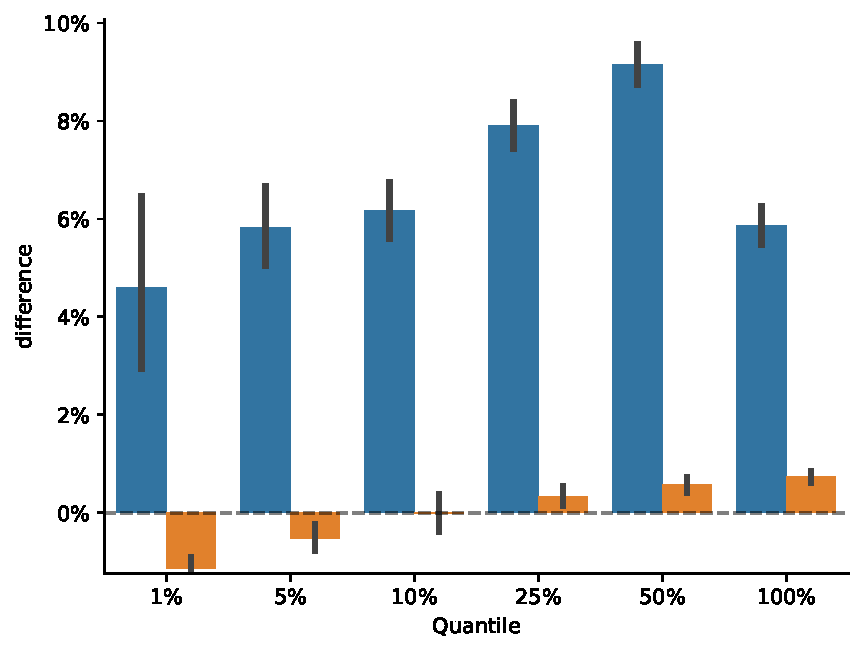
\includegraphics[width=\textwidth]{Figures/train_test_diff_MUTAG.pdf}
		\vspace*{-4ex} 
		\caption{\mutag}
	\end{subfigure}
	\par\bigskip
	\begin{subfigure}[b]{0.3\textwidth}
		\centering
		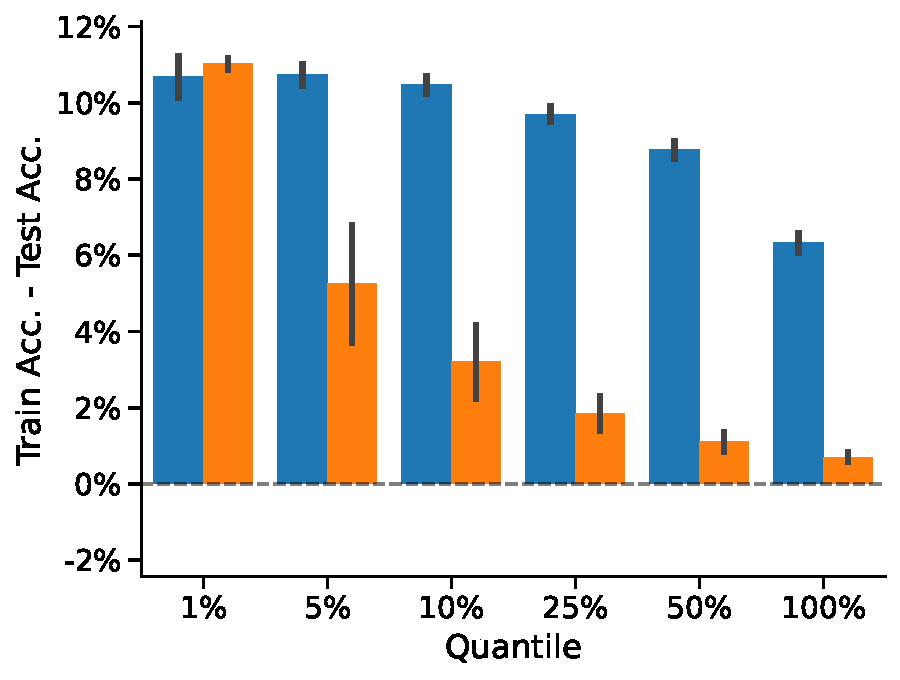
\includegraphics[width=\textwidth]{Figures/train_test_diff_NCI1.pdf}
		\vspace*{-4ex} 
		\caption{\nci}
	\end{subfigure}
	\hfill
	\begin{subfigure}[b]{0.3\textwidth}
		\centering
		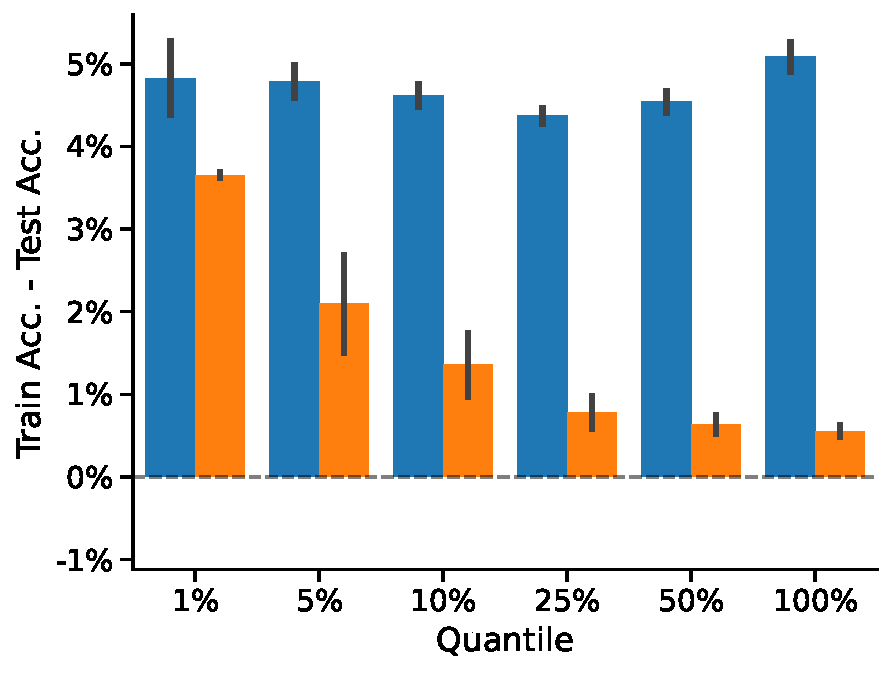
\includegraphics[width=\textwidth]{Figures/train_test_diff_PROTEINS.pdf}
		\vspace*{-4ex} 
		\caption{\proteins}
	\end{subfigure}
	\hfill
	\begin{subfigure}[b]{0.3\textwidth}
		\centering
		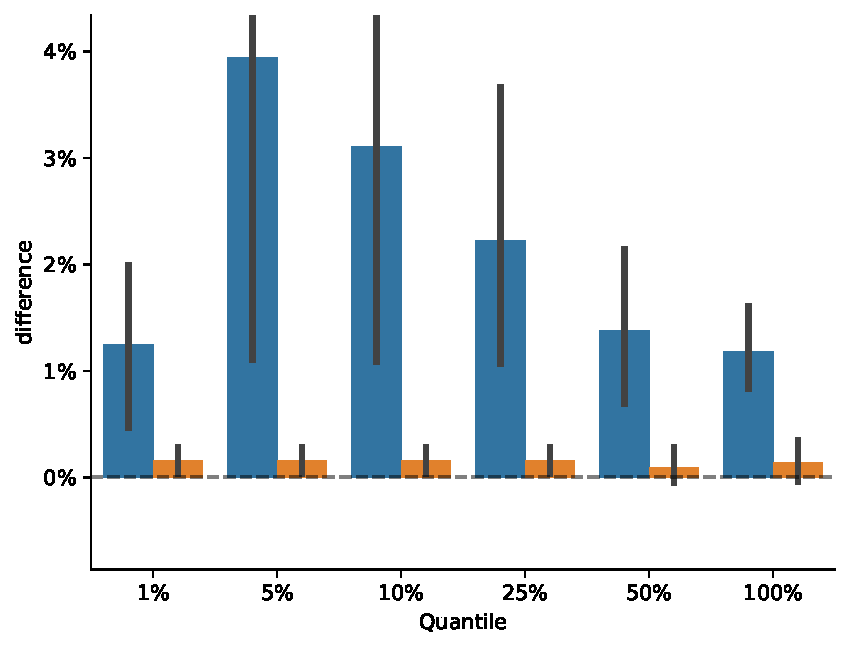
\includegraphics[width=\textwidth]{Figures/train_test_diff_REDDIT-BINARY.pdf}
		\vspace*{-4ex} 
		\caption{\reddit}
	\end{subfigure}
	\centering
	\begin{subfigure}[b]{0.3\textwidth}
		\centering
		
\includegraphics[width=\textwidth]{Figures/train_test_diff_legend.pdf}
		\vspace*{-4ex} 
	\end{subfigure}
	\caption{Mean absolute difference of the classification accuracies of the training and testing set of each dataset. In detail, we compared the different quantiles of each performance.}
	\label{fig:performance_diff}
\end{figure}

Upon analyzing \cref{fig:performance_diff}, it reveals that \wlnn models exhibit more significant overfitting than \gnn models, especially on datasets such as \enzymes, \mutag, \proteins, and \reddit. For instance, in the case of \enzymes, the top \perc{1} of best-performing \wlnn models display, on average, a \perc{27} higher training accuracy than their test accuracy, highlighting the extreme extent of overfitting in \wlnn models.

While \gnn models also experience some overfitting, primarily observed in the \nci dataset, it is not as prevalent across all datasets and not as dramatic as in the case of \wlnn models. Moreover, in datasets like \mutag or \reddit, \gnn models demonstrate superior generalization capability. In these cases, the mean difference in performance is close to \perc{0}, and in the case of Mutag, it is even negative, which indicates that the tested \gnn models were able to learn general patterns in these datasets rather than simply memorizing the data.

However, this raises the question as to why \wlnn models exhibit such dramatic overfitting. We hypothesize that the expressiveness of the \wl algorithm leads to the computation of highly detailed colorings of the \wlnn's input graphs.

To gain insight into the algorithm's expressiveness, we calculated the ratio of unique colors to the total number of possible colors for each classification dataset. For example, the \enzymes dataset consists of 600 graphs with a total of 19\,580 nodes. After a single iteration of the \wl algorithm, all colorings consist of only 231 colors, accounting for less than \perc{0.01} of the total number of possible unique colors (the total number of nodes). However, after two iterations, this number has already increased to 10\,416, comprising \perc{53.2} of the total available colors. This example demonstrates the significant expressiveness of the colorings after just a few iterations.

\begin{figure}[!htb]
	\centering
	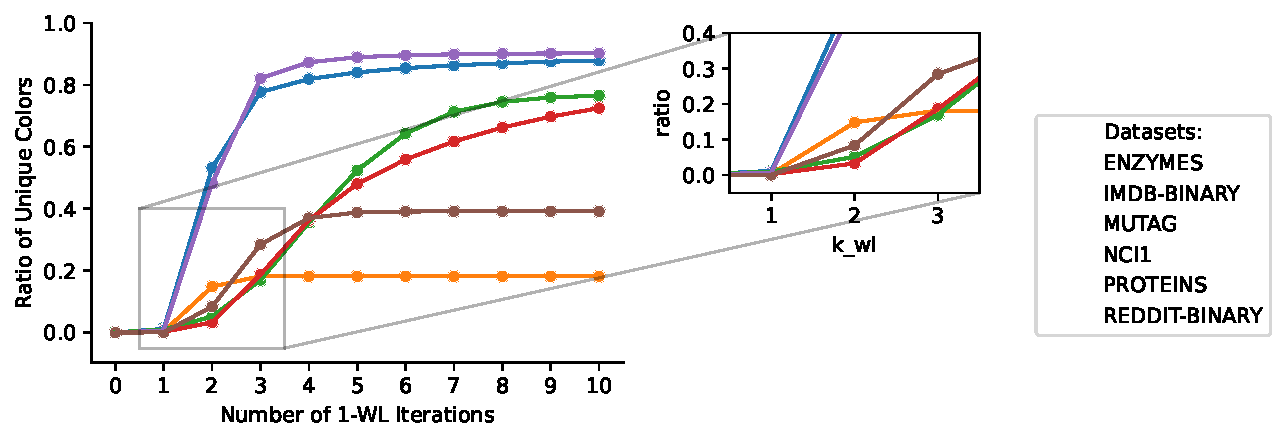
\includegraphics[width=0.975\textwidth]{Figures/wl_unique_colors.pdf}
	\caption{Overview of the ratio of unique colors used by the \wl algorithm when applied for a specified number of iterations for each dataset. The ratios are computed using each dataset's total number of nodes as the maximum number of unique colors that could appear in all colorings.}
	\label{fig:wl_unique_colors}
\end{figure}

\cref{fig:wl_unique_colors} illustrates the ratio of unique colors used compared to the total possible number of unqiue colors (total number of nodes in each dataset). As expected due to the convergence behavior of the \wl algorithm, each ratio convergence at some point. However, the ratios rise rapidly and dramatically for all datasets, indicating the algorithm's expressiveness. Even a relatively small ratio, such as approximately \perc{10}, signifies a significant number of unique colors in the colorings computed by the \wl algorithm. It is important to consider the scale of the datasets when interpreting these ratios. For example, the \mutag dataset consists of approximately 3\,000 nodes, while \enzymes and \imdb datasets contain around 20\,000 nodes each. The \proteins dataset reaches 43\,000 nodes, followed by the \nci dataset with 122\,000 nodes, and finally, the \reddit dataset with a staggering 859\,000 nodes. For a comprehensive overview of the datasets and their sizes, please refer to \cref{tab:overview_datasets}, and for detailed information on the unique color count of each dataset, consult \cref{tab:unique_colors} in the Appendix.

Furthermore, it is important to note that the colors assigned by the \wl algorithm have no inherent structural connection between them. Even if two nodes are colored with two distinct integers that are close together, it does not imply any similarity between them. While our experiments use an implementation of the \wl algorithm that assigns each node the smallest unused color, a meaningful connection between colors is still absent due to shuffling the dataset when applying the \wl algorithm.

To investigate the impact of the number of \wl iterations on overfitting, we plotted \cref{fig:performance_diff_wlnn}, which focuses solely on \wlnn models and compares the different numbers of \wl iterations. Across all classification datasets, it is evident that the overfitting behavior becomes more substantial when increasing the number of \wl iterations. This finding supports our belief that the explosive increase in the number of unique colors is the primary reason for the observed overfitting behavior. In the case of \enzymes, with an increased number of \wl iterations, the average training accuracy is over \perc{60} higher than the test accuracy, demonstrating the worsening of the overfitting behavior.

\begin{figure}[!htb]
	\centering
	\begin{subfigure}[b]{0.3\textwidth}
		\centering
		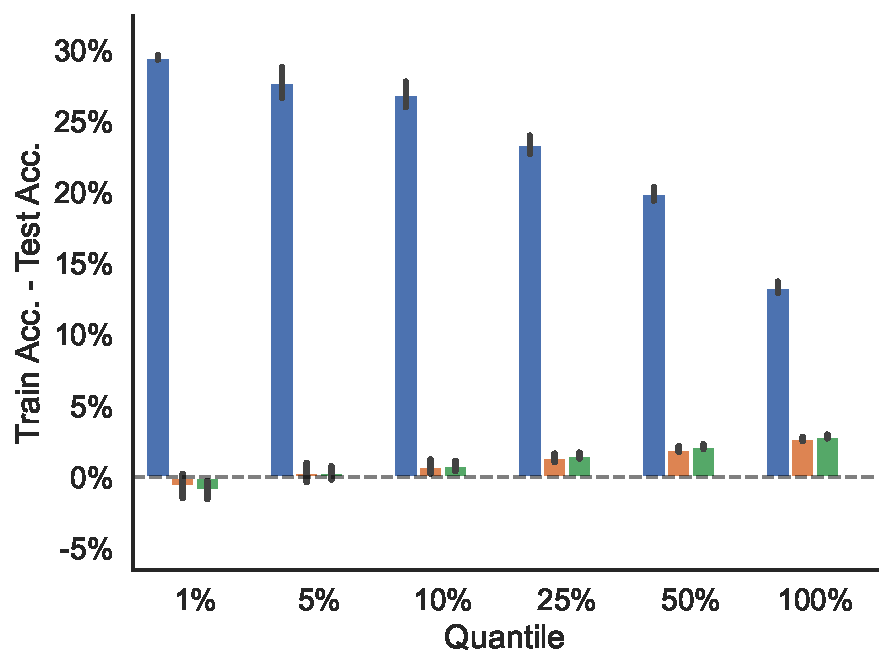
\includegraphics[width=\textwidth]{Figures/train_test_diff_k_wl_ENZYMES.pdf}
		\vspace*{-4ex} 
		\caption{\enzymes}
	\end{subfigure}
	\hfill
	\begin{subfigure}[b]{0.3\textwidth}
		\centering
		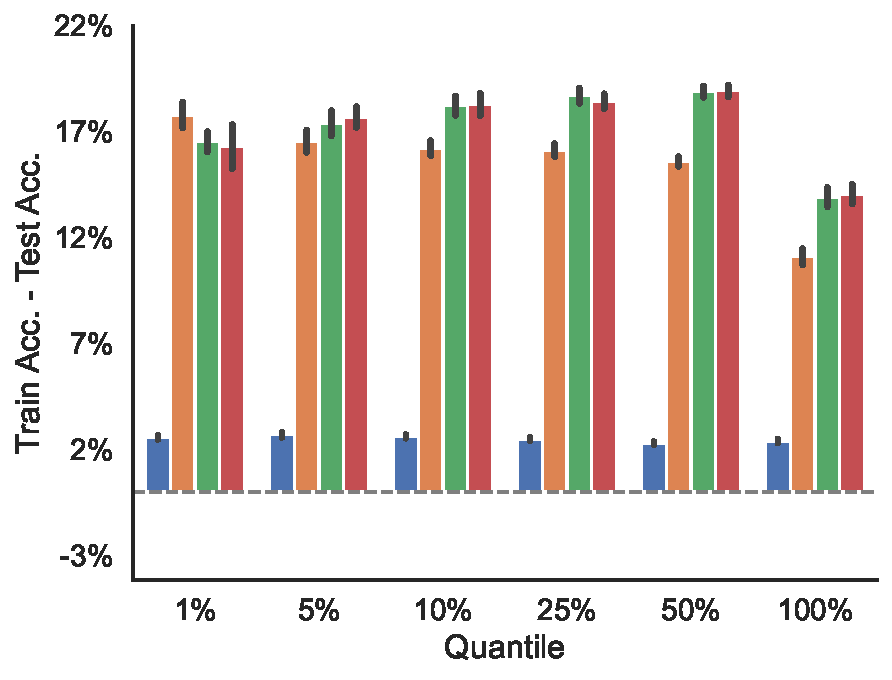
\includegraphics[width=\textwidth]{Figures/train_test_diff_k_wl_IMDB-BINARY.pdf}
		\vspace*{-4ex} 
		\caption{\imdb}
	\end{subfigure}
	\hfill
	\begin{subfigure}[b]{0.3\textwidth}
		\centering
		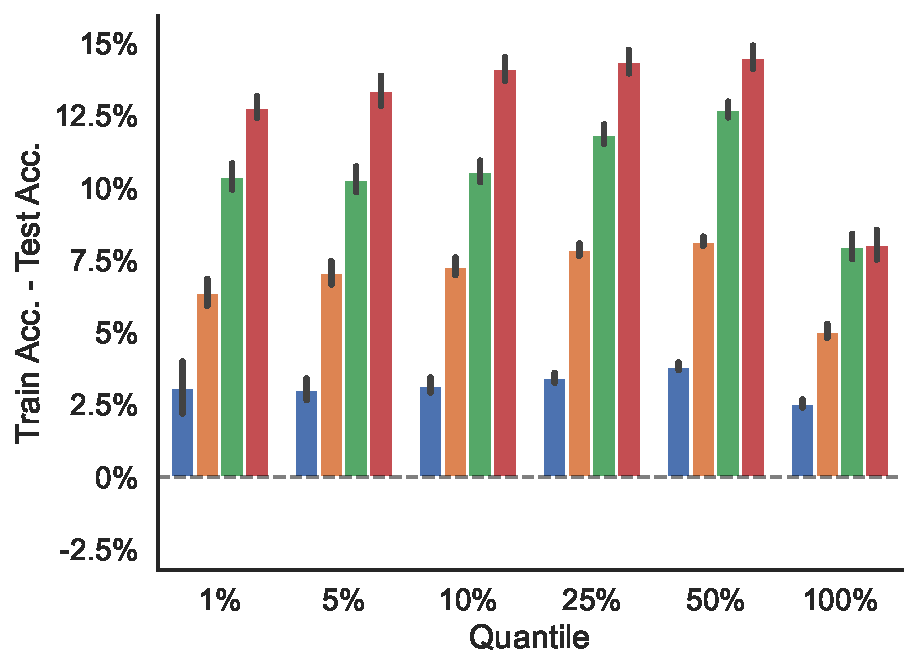
\includegraphics[width=\textwidth]{Figures/train_test_diff_k_wl_MUTAG.pdf}
		\vspace*{-4ex} 
		\caption{\mutag}
	\end{subfigure}
	\par\bigskip
	\begin{subfigure}[b]{0.3\textwidth}
		\centering
		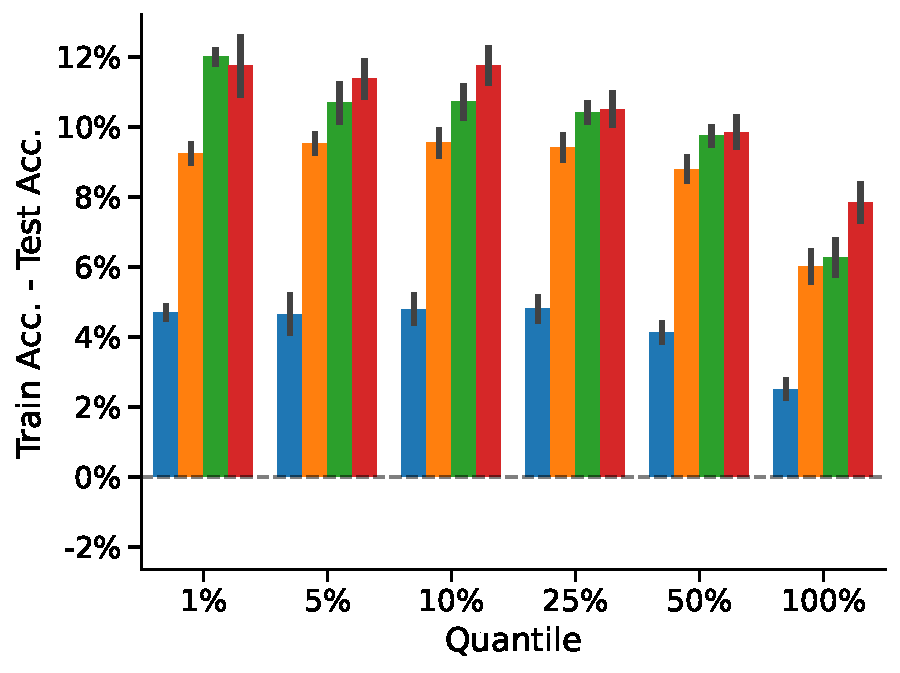
\includegraphics[width=\textwidth]{Figures/train_test_diff_k_wl_NCI1.pdf}
		\vspace*{-4ex} 
		\caption{\nci}
	\end{subfigure}
	\hfill
	\begin{subfigure}[b]{0.3\textwidth}
		\centering
		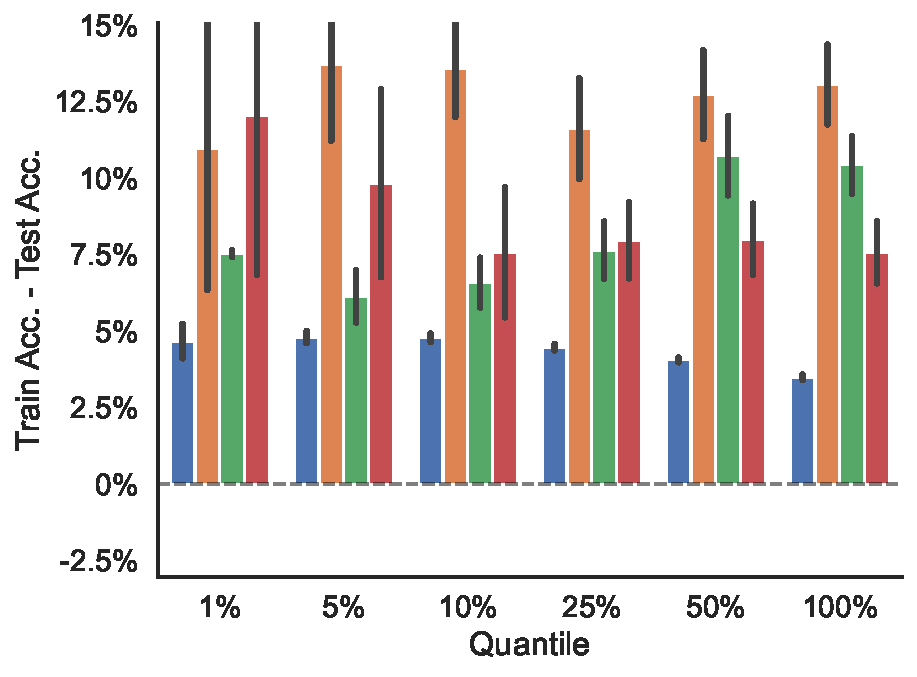
\includegraphics[width=\textwidth]{Figures/train_test_diff_k_wl_PROTEINS.pdf}
		\vspace*{-4ex} 
		\caption{\proteins}
	\end{subfigure}
	\hfill
	\begin{subfigure}[b]{0.3\textwidth}
		\centering
		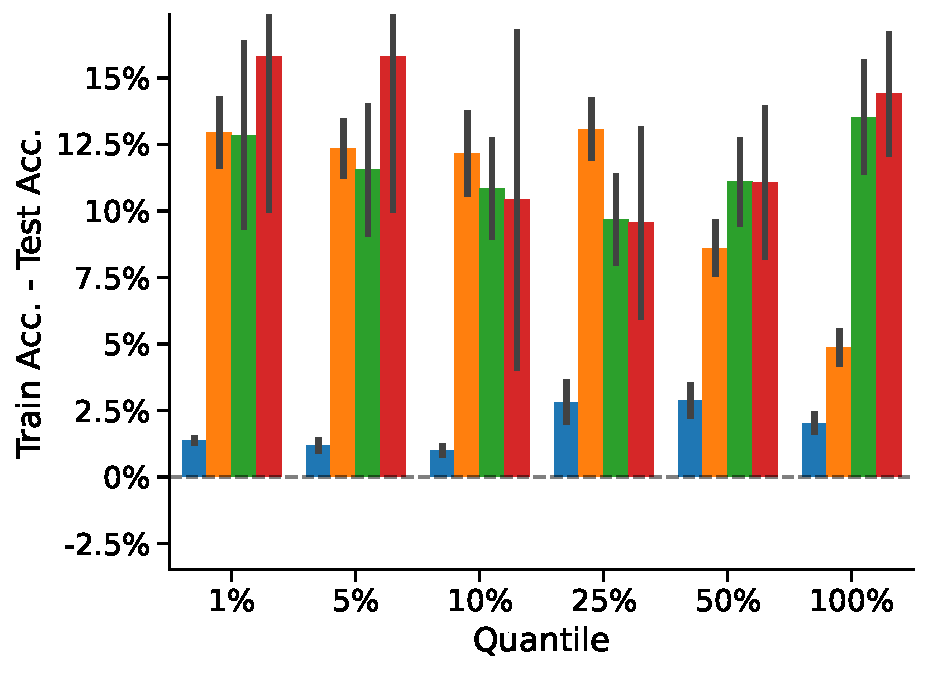
\includegraphics[width=\textwidth]{Figures/train_test_diff_k_wl_REDDIT-BINARY.pdf}
		\vspace*{-4ex} 
		\caption{\reddit}
	\end{subfigure}
	\begin{subfigure}[b]{0.3\textwidth}
		\centering
		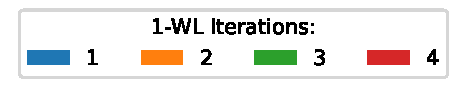
\includegraphics[width=\textwidth]{Figures/train_test_diff_k_wl_legend.pdf}
		\vspace*{-4ex} 
	\end{subfigure}
	\label{fig:performance_diff_wlnn}
\end{figure}

In conclusion, our analysis reveals that \wlnn models exhibit optimal generalization when limited to one iteration of the \wl algorithm. Increasing the number of iterations leads to a significant overfitting behavior. This insight indicates that the expressiveness of the \wl algorithm surpasses the requirements for effective learning. In comparison, \gnn models excel in learning and representing graph structures in a more generalized manner.

Furthermore, our findings suggest that the best-performing \wlnn models, in terms of generalization, are configured using a single \wl iteration. This observation aligns with the results from the previous section, where the models achieving the highest accuracy on the test set also utilized a single iteration of the \wl algorithm (except for the \nci dataset). This observation raises an intriguing question: Do \gnns also attempt to compute a similarly expressive representation of all graphs, akin to a single iteration of the \wl algorithm? We will explore this question in the following section.

\subsection{\gnn Approximating \wl}


\begin{figure}[!htb]
	\centering
	\begin{subfigure}[b]{0.49\textwidth}
		\centering
		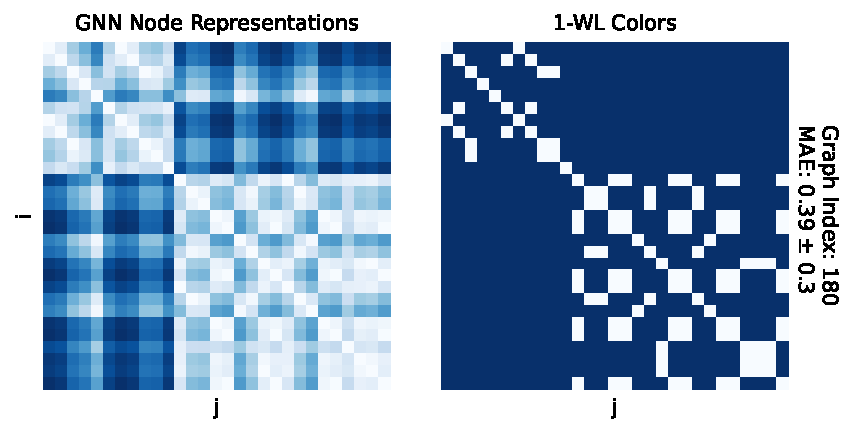
\includegraphics[width=\textwidth]{Figures/heatmaps_ENZYMES_single.pdf}
		\vspace*{-5ex} 
        \caption{\enzymes}
	\end{subfigure}
	\hfill
	\begin{subfigure}[b]{0.49\textwidth}
		\centering
		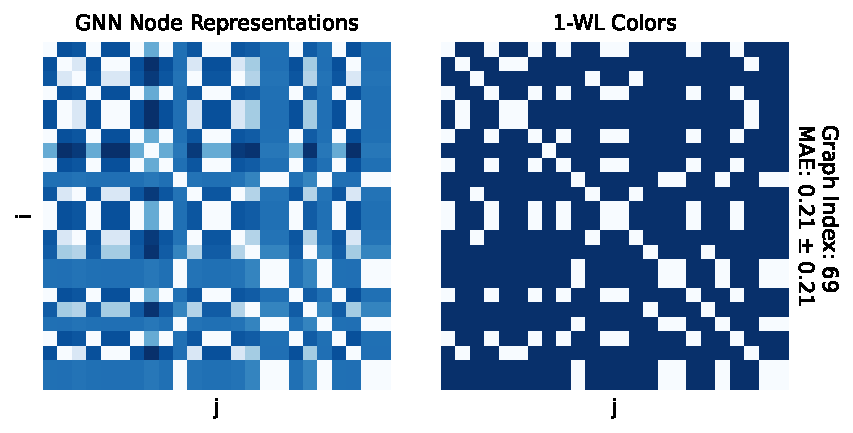
\includegraphics[width=\textwidth]{Figures/heatmaps_IMDB-BINARY_single.pdf}
		\vspace*{-5ex} 
        \caption{\imdb}
	\end{subfigure}
	\par\bigskip
	\begin{subfigure}[b]{0.49\textwidth}
		\centering
		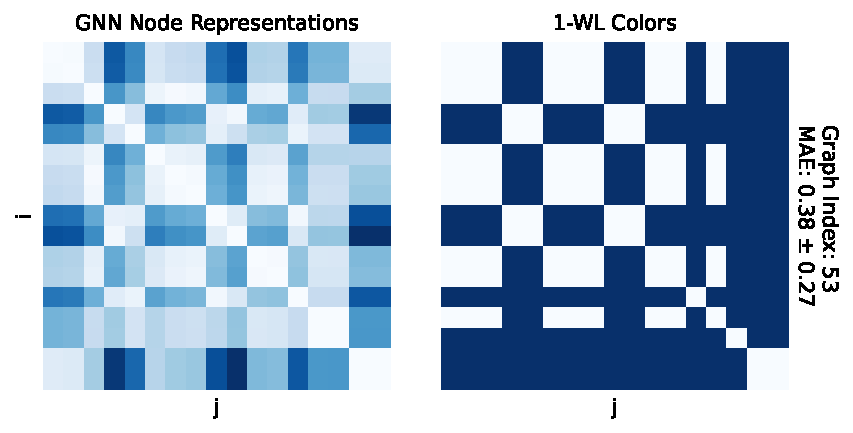
\includegraphics[width=\textwidth]{Figures/heatmaps_MUTAG_single.pdf}
		\vspace*{-5ex} 
        \caption{\mutag}
	\end{subfigure}
	\hfill
	\begin{subfigure}[b]{0.49\textwidth}
		\centering
		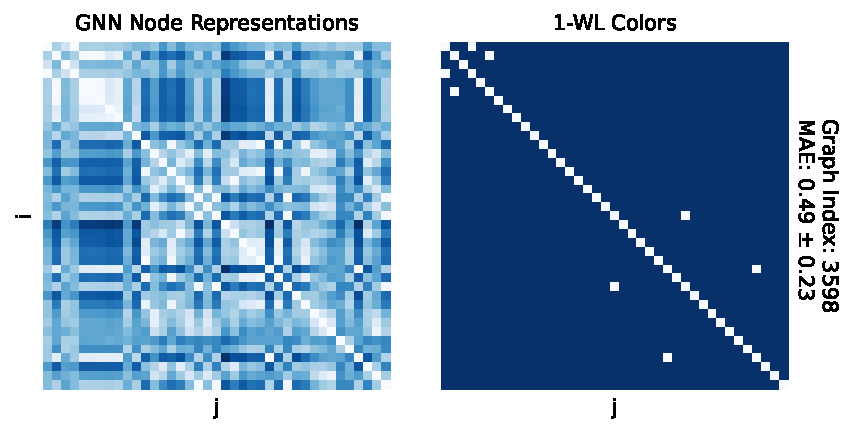
\includegraphics[width=\textwidth]{Figures/heatmaps_NCI1_single.pdf}
		\vspace*{-5ex} 
        \caption{\nci}
	\end{subfigure}
	\par\bigskip
	\begin{subfigure}[b]{0.49\textwidth}
		\centering
		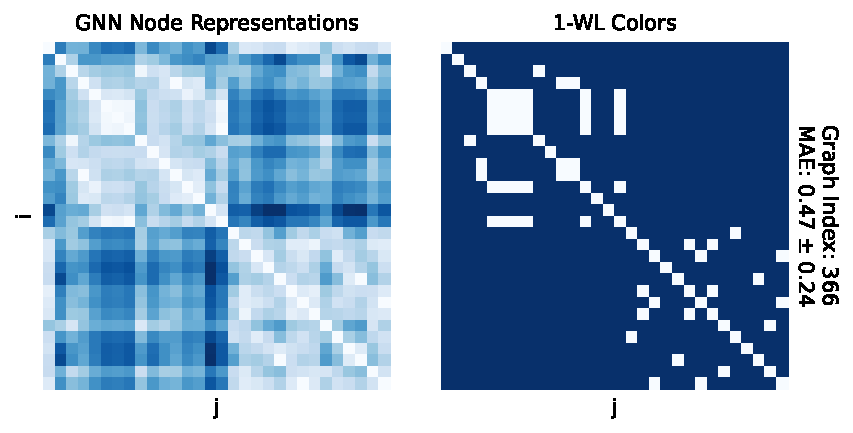
\includegraphics[width=\textwidth]{Figures/heatmaps_PROTEINS_single.pdf}
		\vspace*{-5ex} 
        \caption{\proteins}
	\end{subfigure}
	\hfill
	\begin{subfigure}[b]{0.49\textwidth}
		\centering
		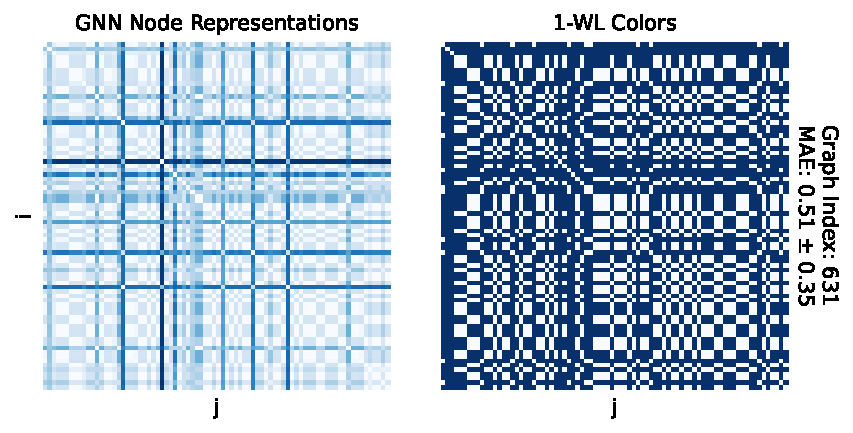
\includegraphics[width=\textwidth]{Figures/heatmaps_REDDIT-BINARY_single.pdf}
		\vspace*{-5ex}
        \caption{\reddit}
	\end{subfigure}
	\par\bigskip
	\begin{subfigure}[t]{0.6\textwidth}
		\centering
		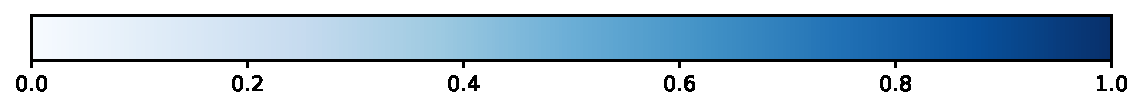
\includegraphics[width=\textwidth]{Figures/colorbar.pdf}
	\end{subfigure}
	\caption{Visualizing the performance of the best-performing \gnn models of each dataset in approximating node colors computed by the \wl algorithm after running for one iteration. Here we randomly sampled a single graph for each dataset and visualized the approximation performance.}
	\label{fig:gnn_approx}
\end{figure}
This section will explore the node features computed by a \gnn. Specifically, we will analyze the ability of \gnns to approximate the coloring computed by a single iteration of the \wl algorithm.

Please refer to \cref{fig:gnn_approx} for a visualization of the approximation capabilities of the best-performing \gnn models evaluated on each classification dataset. For each dataset, we created a pair of color-coded matrices. To construct these matrices, we randomly selected a graph from the test set and calculated the distances between each node in the graph. The left matrix in each pair represents the distance matrix of the node representations computed by the \gnn model, while the matrix on the right represents the distances of the colorings generated by a single iteration of the \wl algorithm. We utilized the Euclidean distance as a measure and subsequently normalized all distances between 0 and 1 for each matrix for the \gnn matrix. Since the colorings produced by the \wl algorithm are discrete and their distances to another do not encoded any information, the distance values are either 0 (for nodes with the same color) or 1 (for nodes with different colors). In addition, we computed the similarity between both matrices using the absolute difference between them and averaged it into a single value (MAE). We included this value along with its standard deviation and the index of the graph in the datasets on the right side of the \wl distance matrix.

From the visualization, it is evident that the \gnn representations already exhibit convincing approximations of the patterns observed in the \wl algorithm's matrix. However, it is important to note that these results are based on a single randomly selected graph from each model's test set. To gain a more comprehensive understanding of the approximation capabilities of each \gnn model, we repeated the process for each dataset using ten randomly selected graphs from the respecitive \gnn models test set. We included their visualizations in the Appendix, in \cref{fig:gnn_approx_enzymes,fig:gnn_approx_imdb,fig:gnn_approx_mutag,fig:gnn_approx_nci_1,fig:gnn_approx_nci_3,fig:gnn_approx_proteins,fig:gnn_approx_reddit}. 

We have to point out that between the node representations computed by a gnn and the colors computed by the \wl algorithm is a significant difference. Compared to the discrete colors, that dont have any order relation between another, the representations computed by each \gnn model are multidimensional and continous. This make a perfect approximation of the \wl colorings hard, as here each representation value computed has a order relation to another, such that defining when two nodes representations are similiar to another is not as straightforward as in discrete \wl case. In our visualization we avoided making this decision by simply normalizing the distanctes uniformaly between 0 and 1 and use a continous colorbar for color coding similar nodes. However, to be able to put these insights we can see visually also in numbers, we used to different approaches: 1.) An evualtion of the approximation using a threshold value for similarity, and 2.) A translation into discrete values and a subswequent evaluation by using the f1 score.

For the first procedure, we defined two node representations as similar if their eucledian distance is less than a threshold $\epsilon$. If this is the case we will set the distance of both nodes to be $0.0$, otherwise we keep the original distance. We repeat this for every node pair in every graph and than compute the Mean absolute errror between this newly devised distance matrix of the \gnn and the \wl coloring distance. We repeat this for every graph in the dataset and average all values into a single new value. By this we weight each graph in the dataset, regardless of its size equally into the final evaluation. We repeated this process for a variety of threshold values $\epsilon$ with $\epsilon \in [0,1]$. See Figure 24 for the Mean Absolute Error for all classification datasets. Note that, since the all distances are normalized, a value of $\epsilon$ close to $1$ would mean that we classifiy the majroity of distance to as neglible. Therefore, we used a log base axis, since the smaller values are more intresting.

The second procedure aims to transform the regression like values into a classificaiton task by and measure how good it classifies if the distance between nodes is significant or not. We do this by introducing a value $\epsilon \in [0, 1]$ such that we classifiy all distance between two node representations with their distance being less than $\epsilon$ as $0$, while all distance greater or equal than $\epsilon$ as $1$. Thereby we are able to derive a distance matrix with discrete values, for which we then use the f1 score to evaluate the approximation capabilty of this mapping. We repeated this process for every graph in a dataset and averaged the f1 score afterward as a final value. Note, that since the number of node pairs that are distinguished by the \wl alogirhtm compared to the number of nodes which are assigned the same color, we have an imbalance between both labels, such that we used the f1 score with the macro weighting to counter any biases in the results. Furthermore, we repeated this process for different $\epsilon$ values. See Figure 25 for the a visualization of the results for each classification dataset.

When analyzing the figures, it is comes immediatly evident that the approximation of the \wl coloring is not perfect, as we can not see a very low mean absolute error neither a very high f1 score for any dataset except for IMDB Binary. Since the dataset IMDB Binar and REDDIT Binary do not have any node features, we utilized the common procedure of initializing their features with an encoding of their node degree. However, for Reddit due to the sheer size of the dataset and its graphs, its maximum node degree is 3062, such that a one\_hot encoding is not useful, for which than utilize a continous node degree encoding which uniformaly maps each node degree into the space $[-1, 1]$. Allthough it holds the same information, only in a continous encoding, we see a clear difference to the discrete one hot encoding employed for IMDB binary which is evident by the significant performance difference between both datasets in our evaluation of the approximation behavior. 

Interestingly, we see a seems to very robust. As can be seen in Figure 4, for epsilon values up to 0.3 the MAE does not change, which leaves us to conclude that the node representations computed by each gnn model for each datasets, maps nodes with different values far away from another in terms of distance, and values that are supposed to be close very far away. This is even more evident, when assesing that the standard deviation for each of graph is very aligned as the deviation is really contained. And since 0.3 is already a very considerable value for setting all distance to less than it to 0.0, we thinkt that the gnn somehow computes a coloring that incorparates essential information of the \wl coloring but leaves out not so important information. As can be seen in the visual representations, the distance between each nodes creates the same patterns as the coloring by the \wl alogirhtm, however not as perfect. And since our \gnn models were able to perform nearly as good as most of the \wlnn models, we conclude that gnn are able to learn a more efficient encoding of their graphs.

Analyzing the other figure, we see that each dataset has its own optimum. However, we still find these optimums in a very close range of the epsilion values between 0.0 and 0.2. Moreover, since almost all datasets achieve a high f1 score we can confirm our believes of the encoding of relevant information. In detail, almost all datasets are able to achieve a score higher than 0.77 except for REDDIT-BINARY. Interestingly, NCI1 is shows exceptional performance with a best mean f1 score of 0.95. This indicates that the node representations computed by the best gnn model for NCI1 is very good at encoding the structural information that can identified with the \wl algorithm using a single iteration very good. Morever, when recalling the dataset taxonomy NCI1 also belongs to the datasets that encodes a lot informaiton in its grpah structures. This is even evidented by us, since NCI1 is the only dataset that seems to perform better with an increased number of \wl iterations for our \wlnn model (see Figure 8).

To why the REDDIT Binary dataset performs so badly in the approximation evalution even though we encode initilize its node features with a node degree encoding and it showing visually good approximation as can be seen in Figure 11 and in Figure 12 in the Appendix, we estimate that it is due to the sheer size of the dataset, in more detail the size of its graph. While all other classification sets have on average arround 30 nodes per graph (including even the regression datasets), REddit Binary has arround 429.6 nodes on average. This means that the number of nodes is significantly larger. Since we the number of message passing layers is fixed for all our gnn models for scalability and comparability to be 5, we assume that gnn models trained on this datasets are not as efficient in propagating messages around the graph, as some information is bound to never be shared with the entire graph just by the number of message passing layers. Allthough this is also evident in other datasets, its is on average not as bad as in reddit binary as evident by the average number of nodes.

In conclusion, we think since \gnn models show similar performance to \wlnn models and since their approximation capabilty of the \wl coloring computed after a single iteration is quite robust but not perfect, we argue that \gnn are able to learn a more efficient encoding of this information. Since both types of frameworks are able to achieve comparable performance on all datasets in terms of accuracies, combined with the insight that most models only utilize a single iteration of the \wl algorithm or an approximation of it for its computation, this begs the question for if this difference can still be seen when pooling this information when using the same pooling function. This question will be investigated in the next session.

\begin{figure}[!htb]
	\centering
	\begin{subfigure}[t]{0.39\textwidth}
		\centering
		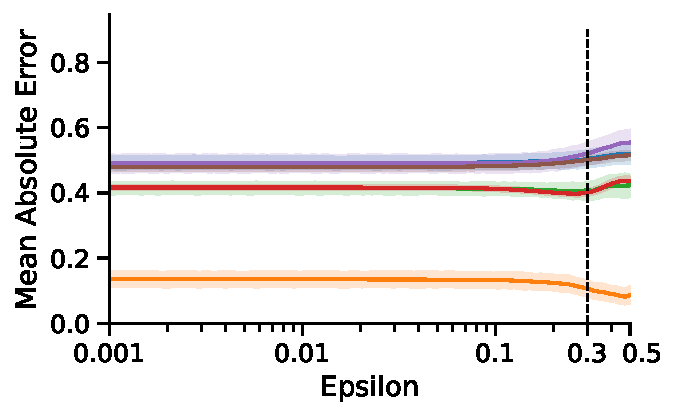
\includegraphics[width=\textwidth]{Figures/global_error_1_b.pdf}
		\caption{Threshold Approximation}
		\label{fig:approx_error}
	\end{subfigure}
	\hfill
	\begin{subfigure}[t]{0.39\textwidth}
		\centering
		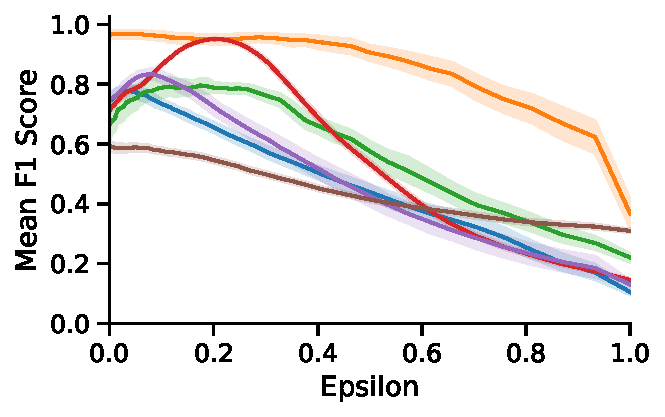
\includegraphics[width=\textwidth]{Figures/global_error_2_b.pdf}
		\caption{F1 Classification Accuracy}
		\label{fig:approx_error_f1}
	\end{subfigure}
	\hfill
	\begin{subfigure}[t]{0.18\textwidth}
		\centering
		\raisebox{22pt}{
			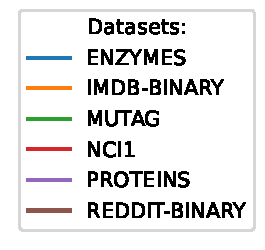
\includegraphics[width=\textwidth]{Figures/global_error_legend.pdf}
		}
		\label{full}%
	\end{subfigure}
	\caption{Error approx with epsilion. Log scale, in a macro mean computation}
	\label{fig:approx_eval}
\end{figure}


\subsection{Preprocessing Data for \gnns}
After learning about the abiltiy of gnns to approximate the coloring of \wl coloring, we further wanted to investigated this topic. Specifically, we wanted to investigate if gnns that are initialized with the the first iteration of the wl colors if they tend to out perform the other.

\subsection{Aggregation Differnces}
Another interesting property we want to investigate is the representation each model derives for a graph. Meaning we anna investigate 

\section{Discusssion}\label{sec:discussion}
\subsection{Learned Lessons}
\subsection{Future Work}

\section{Conclusion}

\newpage


\begin{table}[H]
    \resizebox{.975\textwidth}{!}{ 	\renewcommand{\arraystretch}{1.05}
		\begin{tabular}{@{}c <{\enspace}@{}lcccccc@{}}	\toprule
			& \multirow{3}{*}{\vspace*{4pt}\textbf{Method}}&\multicolumn{6}{c}{\textbf{Dataset}}\\\cmidrule{3-8}
			& & {\enzymes}         &  {\imdb}      & {\mutag}           & {\nci}       & {\proteins}           & 
			{\reddit}
			\\
			\toprule
			\multirow{4}{*}{\rotatebox{90}{$\wlnn$}}
			& \textsf{MLP} & 48.3 \scriptsize	$\pm 8.1$ & \textbf{72.4} \scriptsize	$\pm 4.1$ & 85.1 \scriptsize $\pm 8.6$ & 83.6 \scriptsize	$\pm 4.1$ & \textbf{75.2} \scriptsize $\pm 3.9$ & 78.4 \scriptsize $\pm 2.7$
			\\
			& \textsf{SVM Linear} & 34.4 \scriptsize	$\pm 5.5$ & 71.2 \scriptsize	$\pm 3.9$ & 86.4 \scriptsize $\pm 8.9$	 & 83.4 \scriptsize	$\pm 2.1$ & 73.9 \scriptsize $\pm 4.1$
			\\
			& \textsf{SVM RBF} & 45.0 \scriptsize	$\pm 7.0$ & 72.8 \scriptsize	$\pm 4.3$ & 83.2 \scriptsize $\pm 7.5$ & 83.6 \scriptsize	$\pm 1.9$ & 75.2 \scriptsize $\pm 4.0$
			\\
			& \textsf{k-NN} &  \textbf{56.3} \scriptsize $\pm 5.8$ ($k$=$1$) & 72.3 \scriptsize $\pm 4.1$ ($k$=$11$)& \textbf{86.7} \scriptsize $\pm 7.7$ ($k$=$10$) & \textbf{83.9} \scriptsize $\pm 1.8$ ($k$=$5$)& 73.9 \scriptsize $\pm 4.1$ ($k$=$19$) & 83.2 \scriptsize $\pm 2.5$ ($k$=$13$)
			\\
			\cmidrule{2-8}
			\multirow{4}{*}{\rotatebox{90}{\gnn}}
			& \textsf{MLP} & 34.4 \scriptsize $\pm 7.0$ &  \textbf{74.7} \scriptsize $\pm 3.8$ & 84.6 \scriptsize $\pm 8.7$	 & \textbf{79.9} \scriptsize $\pm 2.2$ & 74.3 \scriptsize $\pm 5.1$ & 86.9 \scriptsize $\pm 3.2$
			\\
			& \textsf{SVM Linear} & 33.2 \scriptsize $\pm 5.9$ & 73.9 \scriptsize $\pm 4.2$ & 51.9 \scriptsize $\pm 34.1$ & 67.4 \scriptsize $\pm 2.2$ & 74.7 \scriptsize $\pm 4.2$
			\\
			& \textsf{SVM RBF} & 35.9 \scriptsize $\pm 6.0$ & 74.1 \scriptsize $\pm 3.9$ & \textbf{86.0} \scriptsize $\pm 7.4$ & 73.0 \scriptsize $\pm 1.9$ & 74.6 \scriptsize $\pm 4.6$
			\\ 
			& \textsf{k-NN} & \textbf{51.6} \scriptsize $\pm 7.0$ ($k$=$1$)	& 74.3 \scriptsize $\pm 4.0$ ($k$=$132$) & 88.3 \scriptsize $\pm 6.5$ ($k$=$38$) & 77.5 \scriptsize $\pm 1.7$ ($k$=$2$)& \textbf{74.9} \scriptsize $\pm 4.3$ ($k$=$27$) & 90.8 \scriptsize $\pm 1.8$ ($k$=$15$)
			\\
			\bottomrule
		\end{tabular}}
		\caption{Overview of the classification accuracies achieved by the best model for each dataset in percent and standard deviation. Additionally, the performance of each model was evaluated under alternative configurations, namely the substitution of the Multilayer Perceptron (MLP) with a Support Vector Machine employing either a linear kernel (SVM Linear) or the Radial Basis Function (SVM RBF), as well as the k-nearest neighbors algorithm (k-NN) with different values for $k$.}
        \label{tab:my_label3}                  
\end{table}

\begin{figure}[H]
	\begin{subfigure}[b]{0.3\textwidth}
		\centering
		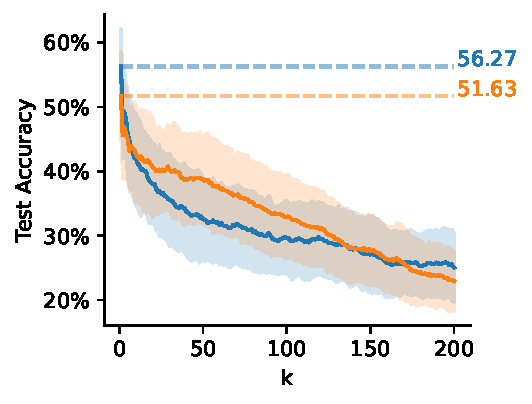
\includegraphics[width=\textwidth]{Figures/knn_ENZYMES.pdf}
		\vspace*{-4ex} 
		\caption{\enzymes}
	\end{subfigure}
	\hfill
	\begin{subfigure}[b]{0.3\textwidth}
		\centering
		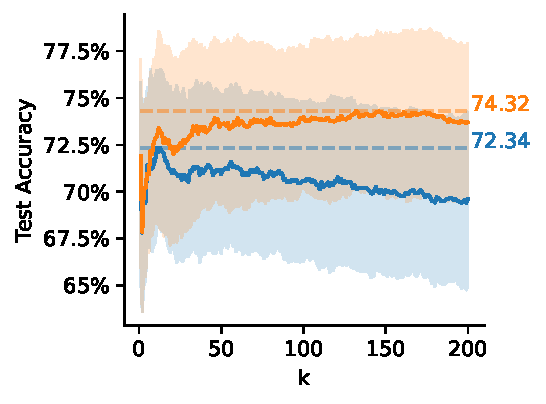
\includegraphics[width=\textwidth]{Figures/knn_IMDB-BINARY.pdf}
		\vspace*{-4ex} 
		\caption{\imdb}
	\end{subfigure}
	\hfill
	\begin{subfigure}[b]{0.3\textwidth}
		\centering
		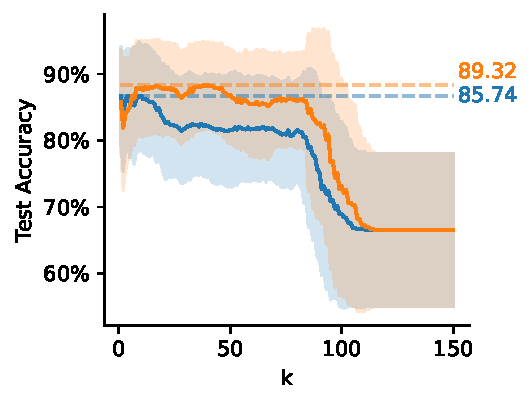
\includegraphics[width=\textwidth]{Figures/knn_MUTAG.pdf}
		\vspace*{-4ex} 
		\caption{\mutag}
	\end{subfigure}
	\par\bigskip
	\begin{subfigure}[b]{0.3\textwidth}
		\centering
		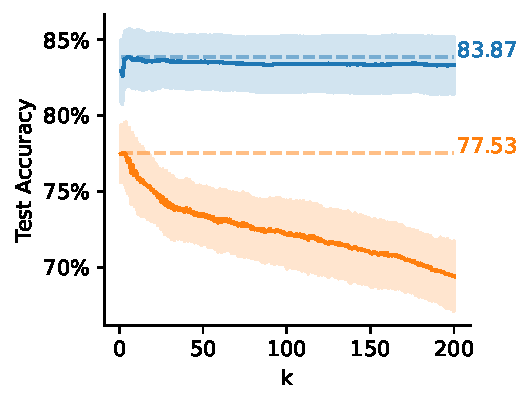
\includegraphics[width=\textwidth]{Figures/knn_NCI1.pdf}
		\vspace*{-4ex} 
		\caption{\nci}
	\end{subfigure}
	\hfill
	\begin{subfigure}[b]{0.3\textwidth}
		\centering
		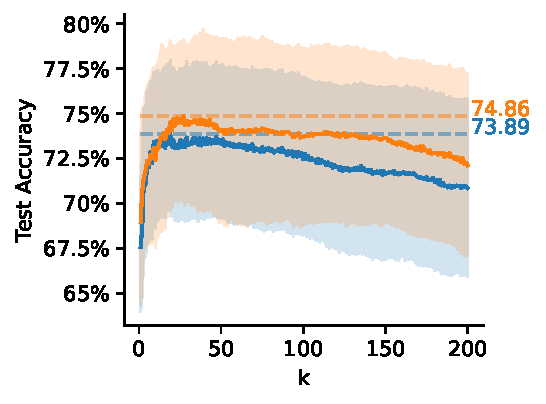
\includegraphics[width=\textwidth]{Figures/knn_PROTEINS.pdf}
		\vspace*{-4ex} 
		\caption{\proteins}
	\end{subfigure}
	\hfill
	\begin{subfigure}[b]{0.3\textwidth}
		\centering
		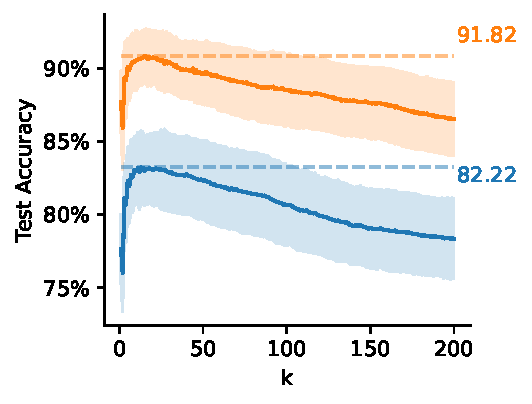
\includegraphics[width=\textwidth]{Figures/knn_REDDIT-BINARY.pdf}
		\vspace*{-4ex} 
		\caption{\reddit}
	\end{subfigure}
	\centering
	\begin{subfigure}[b]{0.3\textwidth}
		\centering
		
\includegraphics[width=\textwidth]{Figures/train_test_diff_legend.pdf}
		\vspace*{-4ex} 
	\end{subfigure}
	\caption{Average classification accuracy achieved on each dataset by replacing the multilayer perceptron of the best-performing \wlnn and \gnn model with a classifier based on the $k$-nearest neighbors algorithm. We tested for different values of $k$.}
\end{figure}

\begin{figure}[H]
	\begin{subfigure}[b]{0.49\textwidth}
		\centering
		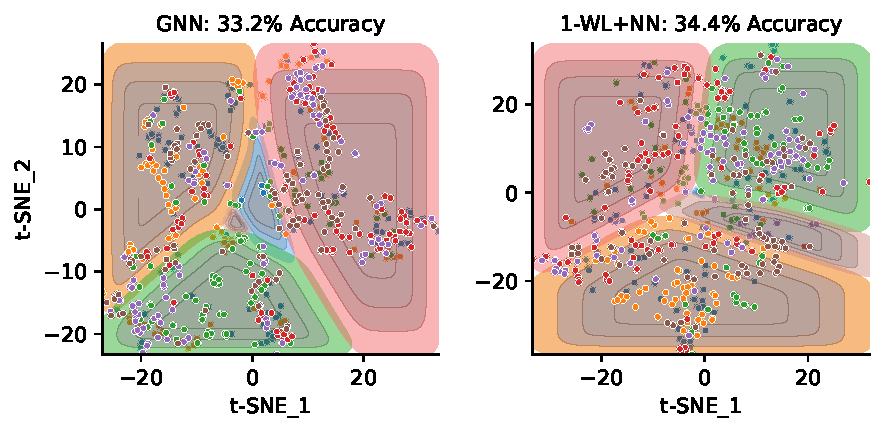
\includegraphics[width=\textwidth]{Figures/tsne_svm_lin_ENZYMES.pdf}
		\vspace*{-4ex} 
		\caption{\enzymes}
	\end{subfigure}
	\hfill
	\begin{subfigure}[b]{0.49\textwidth}
		\centering
		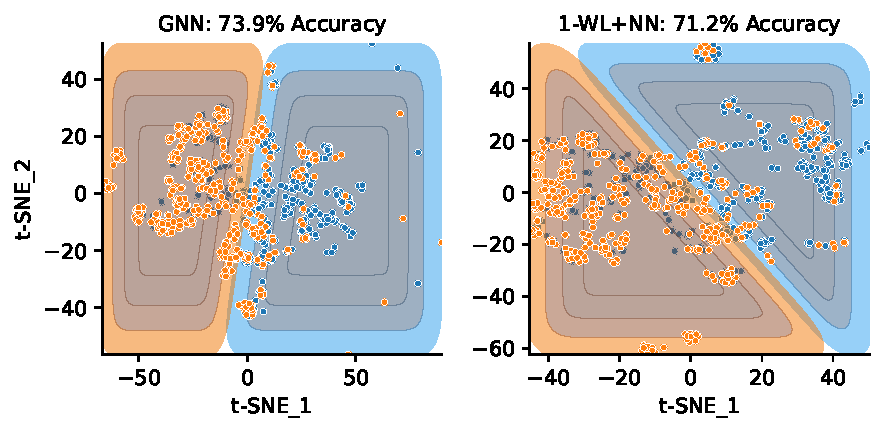
\includegraphics[width=\textwidth]{Figures/tsne_svm_lin_IMDB.pdf}
		\vspace*{-4ex} 
		\caption{\imdb}
	\end{subfigure}
	\par\bigskip
	\begin{subfigure}[b]{0.49\textwidth}
		\centering
		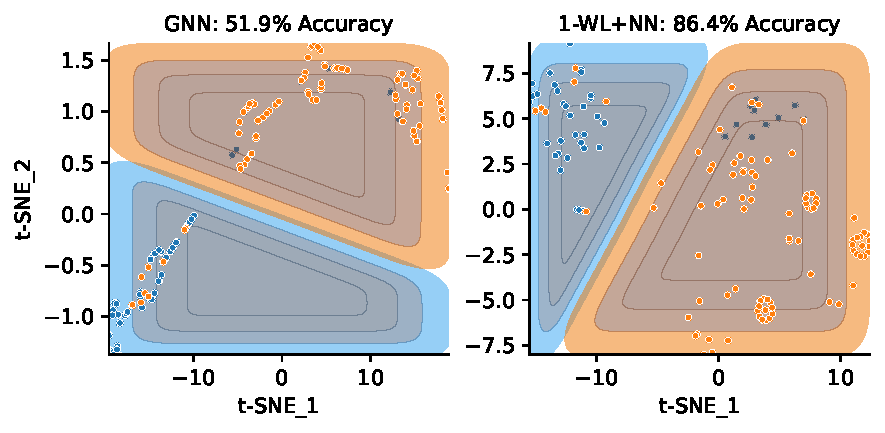
\includegraphics[width=\textwidth]{Figures/tsne_svm_lin_MUTAG.pdf}
		\vspace*{-4ex} 
		\caption{\mutag}
	\end{subfigure}
	\hfill
	\begin{subfigure}[b]{0.49\textwidth}
		\centering
		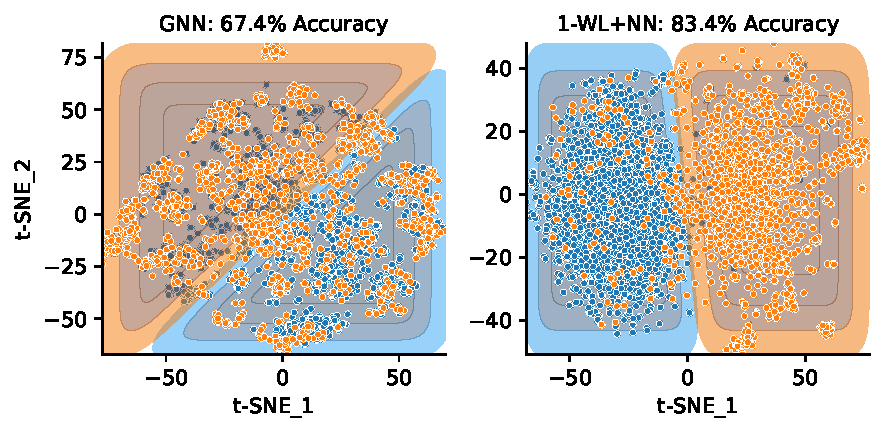
\includegraphics[width=\textwidth]{Figures/tsne_svm_lin_NCI1.pdf}
		\vspace*{-4ex} 
		\caption{\nci}
	\end{subfigure}
	\par\bigskip
	\begin{subfigure}[b]{0.49\textwidth}
		\centering
		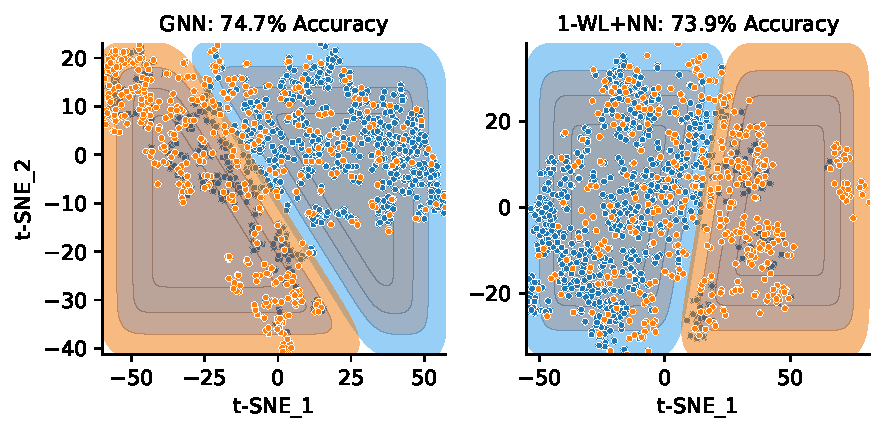
\includegraphics[width=\textwidth]{Figures/tsne_svm_lin_PROTEINS.pdf}
		\vspace*{-4ex} 
		\caption{\proteins}
	\end{subfigure}
	\hfill
	\begin{subfigure}[b]{0.49\textwidth}
		\centering
		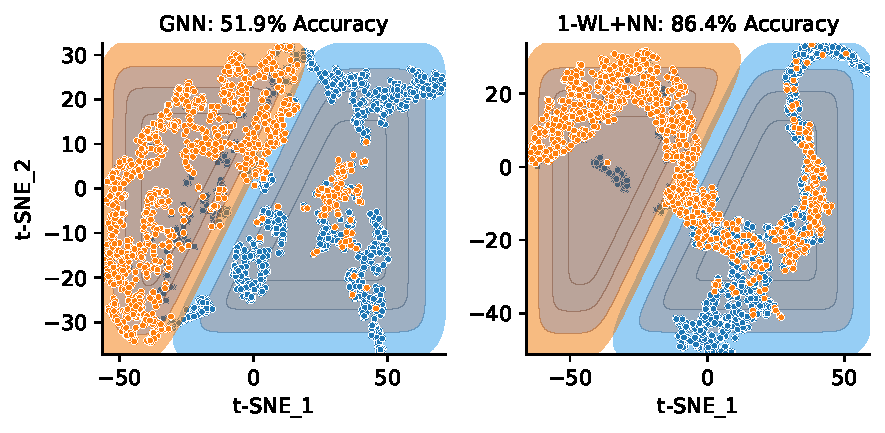
\includegraphics[width=\textwidth]{Figures/tsne_svm_lin_REDDIT.pdf}
		\vspace*{-4ex} 
		\caption{\reddit}
	\end{subfigure}
	\caption{Visualization of the decision boundary of each Support Vector Machine with a linear kernel using t-SNE.}
\end{figure}